

%%%%%%%%%%%%%%%%%%%%%%%%%%%%%%%%%%%%%%%%%%%%%%%%%%%%%%%%%%%%%%%
% Como o modelo faz o uso do bibtex para as referências,
% quando as mesmas são alteradas, quando as citações são
% alteradas, dentre outros casos, é necessário recompilar
% o bibtex. Para isso, siga a ordem de compilação (apenas 
% nos casos citados acima):
%
% (pdf)latex + bibtex + (pdf)latex + (pdf)latex [+ preview]
%
% sendo que o comando [+ preview] é opcional para a 
% visualização do documento.
% No editor TexMaker, as teclas de atalho para os comandos
% acima são:
%
% F6 + F11 + F6 + F6 [+ F7]
%
% Observação: Você pode fazer isso alterando as configurações
%             em "Opções -> Configurar o TexMaker", onde na
%             janela de configuração, na barra lateral,
%             selecione Compilar, altere o campo "Comandos
%             de Compilação Rápida" para o segundo (que
%             que parece com os comandos acima) e dê ok.
%             Use a opção "Compilar" do TexMaker agora que
%             a ordem de comandos acima será executada,
%             gerando, assim, as referências.
%%%%%%%%%%%%%%%%%%%%%%%%%%%%%%%%%%%%%%%%%%%%%%%%%%%%%%%%%%%%%%%

\documentclass[
	% -- opções da classe memoir --
	12pt,				% tamanho da fonte
	openright,			% capítulos começam em pág ímpar (insere página vazia caso preciso)
    twoside,			% para impressão em recto e verso. Oposto a oneside
	a4paper,			% tamanho do papel.
	% -- opções da classe abntex2 --
	%chapter=TITLE,		% títulos de capítulos convertidos em letras maiúsculas
	%section=TITLE,		% títulos de seções convertidos em letras maiúsculas
	%subsection=TITLE,	% títulos de subseções convertidos em letras maiúsculas
	%subsubsection=TITLE,% títulos de subsubseções convertidos em letras maiúsculas
	% -- opções do pacote babel --
	english,			% idioma adicional para hifenização
	french,				% idioma adicional para hifenização
	spanish,			% idioma adicional para hifenização
	brazil				% o último idioma é o principal do documento
	]{abntex2}

% ---
% Pacotes básicos 
% ---
\usepackage{lmodern}			% Usa a fonte Latin Modern			
\usepackage[T1]{fontenc}		% Selecao de codigos de fonte.
\usepackage[utf8]{inputenc}		% Codificacao do documento (conversão automática dos acentos)
\usepackage{lastpage}			% Usado pela Ficha catalográfica
\usepackage{indentfirst}		% Indenta o primeiro parágrafo de cada seção.
% Pacote para o uso de cores no documento
\usepackage{color}
% Pacote para a inclusão\manipulação de imagens
\usepackage{graphicx}
\usepackage{microtype} 			% para melhorias de justificação
% ---
		
% ---
% Pacotes adicionais, usados apenas no âmbito do Modelo Canônico do abnteX2
% ---
\usepackage{lipsum}				% para geração de dummy text
% ---

% ---
% Pacotes para escrita matemática
% ---
\usepackage{amsmath}

\usepackage{amssymb}	 % qed
\usepackage{amsthm}      % Teoremas

\newenvironment{amatrix}[1]{%
  \left(\begin{array}{@{}*{#1}{c}|c@{}}
}{%
  \end{array}\right)
}

% Cria um novo ambiente para Teorema
\newtheorem{teorema}{Teorema}
% Cria um novo ambiente para Definição
\newtheorem{definicao}{Definição}
% Cria um novo ambiente para Exemplo
\newtheorem{exemplo}{Exemplo}
% Cria um novo ambiente para Lema
\newtheorem{lema}{Lema}
%%%%%%%%%%%%%%%%%%%%%%%%%%%%%%%%%%%%%%%%%%%%%%%%%%%%%%%%%%%%%%%
% Recria o ambiente para demonstrações
% \begin{proof} [...] \end{proof}
% 			Observação: O ambiente foi recriado para adequação
%						das fontes com o restante do texto
%%%%%%%%%%%%%%%%%%%%%%%%%%%%%%%%%%%%%%%%%%%%%%%%%%%%%%%%%%%%%%%
\makeatletter
\renewenvironment{proof}[1][\proofname]{
	\par\pushQED{\qed}%
	\normalfont \topsep6\p@\@plus6\p@\relax
	\trivlist
	\item\relax
		{\itshape
			#1\@addpunct{.}}\hspace\labelsep\ignorespaces
}{%
	\popQED\endtrivlist\@endpefalse
}
\makeatother

% Reseta o numerador do ambiente Lema ao fim de todo
% capítulo. Assim, os Lemas serão indexados por capítulo
% e não no documento todo. Por exemplo, no Capítulo 1,
% tem-se, Lema 1.1, Lema 1.2, etc.
\numberwithin{lema}{chapter}
% Mesma função explicada acima para os ambientes de
% teorema, definição, exemplo, figure
\numberwithin{teorema}{chapter}
\numberwithin{definicao}{chapter}
\numberwithin{exemplo}{chapter}
\numberwithin{figure}{chapter}

% Pacotes do Tikz utilizados para desenho
\usepackage{tikz, tkz-euclide, tkz-fct}
\usetikzlibrary{babel}
\usetkzobj{all}

% Pacote para a inclusão de códigos e para gerar
% "Syntax Highlight" (Coloração do Código)
\usepackage{listings}


% Define o nome de marcação para os Blocos de Código
\renewcommand{\lstlistingname}{Código}
% Define o nome de marcação para a Lista de Códigos
\renewcommand{\lstlistlistingname}{Lista de \lstlistingname s}
% Comandos utilizados para a criação e estilização
% da Lista de Códigos
\begingroup\makeatletter
\let\newcounter\@gobble\let\setcounter\@gobbletwo
	\globaldefs\@ne \let\c@loldepth\@ne
	\newlistof{listings}{lol}{\lstlistlistingname}
	\newlistentry{lstlisting}{lol}{0}
\endgroup
\renewcommand{\cftlstlistingaftersnum}{\hfill--\hfill}
% Comandos para a recriação do comando \lstlistoflistings,
% ou seja, para criar a Lista de Códigos
\let\oldlstlistoflistings\lstlistoflistings
\renewcommand{\lstlistoflistings}{%
	\begingroup%
	\let\oldnumberline\numberline%
	\renewcommand{\numberline}{\lstlistingname\space\oldnumberline}%
	\oldlstlistoflistings%
	\endgroup}
% Cria um novo estilo de formatação de código
% para a Linguagem de programação Python
% a ser utilizada no ambiente "lstlisting".
\lstdefinestyle{Python}{
	language={Python},
	basicstyle=\ttfamily\small,
	identifierstyle=\color{black},
	keywordstyle=\color{blue},
	commentstyle=\color{green},
	stringstyle=\color{red},
	extendedchars=true,
	showspaces=false,
	showstringspaces=false,
	numbers=none,
	breaklines=true,
	backgroundcolor=\color{yellow!20},
	breakautoindent=true,
	captionpos=b,
	xleftmargin=0pt,
	frame=none
}

\usepackage{subcaption}

% ---
% Pacotes de citações
% ---
\usepackage[brazilian,hyperpageref]{backref}	 % Paginas com as citações na bibl
% Pacote abntex2cite para citações no padrão ABNT
\usepackage[alf]{abntex2cite}
% --- 
% CONFIGURAÇÕES DE PACOTES
% --- 

% ---
% Configurações do pacote backref
% Usado sem a opção hyperpageref de backref
\renewcommand{\backrefpagesname}{Citado na(s) página(s):~}
% Texto padrão antes do número das páginas
\renewcommand{\backref}{}
% Define os textos da citação
\renewcommand*{\backrefalt}[4]{
	\ifcase #1 %
		Nenhuma citação no texto.%
	\or
		Citado na página #2.%
	\else
		Citado #1 vezes nas páginas #2.%
	\fi}%
% ---

% ---
% Informações de dados para CAPA e FOLHA DE ROSTO
% ---
\titulo{\textbf{Cálculo Variacional}}
\autor{EDUARDO JOSÉ DE OLIVEIRA}
\local{Anápolis}
\data{2019}
\orientador{Prof. Me. Tiago de Lima Bento Pereira}
%\coorientador{Titulação e Nome do coorientador}
\instituicao{%
Universidade Estadual de Goiás
  \par
Câmpus Anápolis de Ciências Exatas e Tecnológicas Henrique Santillo
  \par
Curso de Matemática}
\tipotrabalho{Trabalho de Curso (Graduação)}
% O preambulo deve conter o tipo do trabalho, o objetivo, 
% o nome da instituição e a área de concentração 
\preambulo{Trabalho de Curso (TC) apresentado a Coordenação Adjunta de TC, como parte dos requisitos para obtenção do título de Graduado no Curso de Matemática da Universidade Estadual de Goiás.} %sob a orientação do Professor(a) titulação e nome do professor(a).}
% ---


% ---
% Configurações de aparência do PDF final

% alterando o aspecto da cor azul
\definecolor{blue}{RGB}{41,5,195}

% informações do PDF
\makeatletter
\hypersetup{
     	%pagebackref=true,
		pdftitle={\@title}, 
		pdfauthor={\@author},
    	pdfsubject={\imprimirpreambulo},
	    pdfcreator={LaTeX with abnTeX2},
		pdfkeywords={abnt}{latex}{abntex}{abntex2}{trabalho acadêmico}, 
		colorlinks=false,       		% false: boxed links; true: colored links
    	linkcolor=blue,          	% color of internal links
    	citecolor=blue,        		% color of links to bibliography
    	filecolor=magenta,      		% color of file links
		urlcolor=blue,
		bookmarksdepth=4
}
\makeatother
% --- 

% Define o tamanho da indentação do paragrafo
\setlength{\parindent}{1.5cm}
% Define o espaçamento entre um parágrafo e outro
\setlength{\parskip}{0.2cm}

% Customizações para o Curso de Matemática do Campus CET
% da Universidade Estadual de Goiás.
\usepackage{abntex2matematicaCCET}

% Pacote genealogytree. Usado apenas para os símbolos de
% nascimento e morte, usados nessas datas no capítulo
% sobre história.
\usepackage{genealogytree}
% Cria um comando utilizado para inserir a data de nascimento
% e morte como nota de rodapé.
\newcommand{\bdDate}[2]{
	\footnote{\gtrsymBorn\text{ }#1 - \gtrsymDied\text{ }#2}
}


\usepackage{mathptmx}
\renewcommand{\ABNTEXchapterfont}{\normalfont}

% 
\usepackage{pdfpages}

% ---
% compila o indice
% ---
\makeindex

\begin{document}


% Seleciona o idioma do documento (conforme pacotes do babel)
%\selectlanguage{english}
\selectlanguage{brazil}

% Retira espaço extra obsoleto entre as frases.
\frenchspacing 

%\sffamily

% ----------------------------------------------------------
% ELEMENTOS PRÉ-TEXTUAIS
% ----------------------------------------------------------
\pretextual

% ---
% Capa
% ---

\imprimircapa
% ---

% ---
% Folha de rosto
% (o * indica que haverá a ficha bibliográfica)
% ---
\imprimirfolhaderosto*
% ---

% ---
% Inserir a ficha bibliografica
% ---

% Isto é um exemplo de Ficha Catalográfica, ou ``Dados internacionais de
% catalogação-na-publicação''. Você pode utilizar este modelo como referência. 
% Porém, provavelmente a biblioteca da sua universidade lhe fornecerá um PDF
% com a ficha catalográfica definitiva após a defesa do trabalho. Quando estiver
% com o documento, salve-o como PDF no diretório do seu projeto e substitua todo
% o conteúdo de implementação deste arquivo pelo comando abaixo:
%
% \begin{fichacatalografica}
%     \includepdf[pages=1]{fig_ficha_catalografica.pdf}
% \end{fichacatalografica}

\begin{fichacatalografica}
	\sffamily
	\vspace*{\fill}					% Posição vertical
	\begin{center}					% Minipage Centralizado
	\fbox{\begin{minipage}[c][8cm]{13.5cm}		% Largura
	\small
	\imprimirautor
	%Sobrenome, Nome do autor
	
	\hspace{0.5cm} \imprimirtitulo  / \imprimirautor. --
	\imprimirlocal, \imprimirdata-
	
	\hspace{0.5cm} \pageref{LastPage} p. : il. (algumas color.) ; 30 cm.\\
	
	\hspace{0.5cm} \imprimirorientadorRotulo~\imprimirorientador\\
	
	\hspace{0.5cm}
	\parbox[t]{\textwidth}{\imprimirtipotrabalho~--~\imprimirinstituicao,
	\imprimirdata.}\\
	
	\hspace{0.5cm}
		1. Palavra-chave1.
		2. Palavra-chave2.
		2. Palavra-chave3.
		I. Orientador.
		II. Universidade xxx.
		III. Faculdade de xxx.
		IV. Título 			
	\end{minipage}}
	\end{center}
\end{fichacatalografica}
% ---

\iffalse
% ---
% Inserir errata
% ---
\begin{errata}
Elemento opcional da \citeonline[4.2.1.2]{NBR14724:2011}. Exemplo:

\vspace{\onelineskip}

FERRIGNO, C. R. A. \textbf{Tratamento de neoplasias ósseas apendiculares com
reimplantação de enxerto ósseo autólogo autoclavado associado ao plasma
rico em plaquetas}: estudo crítico na cirurgia de preservação de membro em
cães. 2011. 128 f. Tese (Livre-Docência) - Faculdade de Medicina Veterinária e
Zootecnia, Universidade de São Paulo, São Paulo, 2011.

\begin{table}[htb]
\center
\footnotesize
\begin{tabular}{|p{1.4cm}|p{1cm}|p{3cm}|p{3cm}|}
  \hline
   \textbf{Folha} & \textbf{Linha}  & \textbf{Onde se lê}  & \textbf{Leia-se}  \\
    \hline
    1 & 10 & auto-conclavo & autoconclavo\\
   \hline
\end{tabular}
\end{table}

\end{errata}
% ---
\fi

% ---
% Inserir folha de aprovação
% ---

% Isto é um exemplo de Folha de aprovação, elemento obrigatório da NBR
% 14724/2011 (seção 4.2.1.3). Você pode utilizar este modelo até a aprovação
% do trabalho. Após isso, substitua todo o conteúdo deste arquivo por uma
% imagem da página assinada pela banca com o comando abaixo:
%
% \includepdf{folhadeaprovacao_final.pdf}
%
\begin{folhadeaprovacao}

  \begin{center}
  {\ABNTEXchapterfont\bfseries\large\imprimirtitulo}
%    {\ABNTEXchapterfont\large\imprimirautor}

    \vspace*{\fill}\vspace*{\fill}
    \begin{center}
    {\ABNTEXchapterfont\large\imprimirautor}
%      \ABNTEXchapterfont\bfseries\Large\imprimirtitulo
    \end{center}
    \vspace*{\fill}
    
%    \hspace{.45\textwidth}
%    \begin{minipage}{.5\textwidth}
%        \imprimirpreambulo
%    \end{minipage}%
%    \vspace*{\fill}
\end{center}
\vfill  
      
   Trabalho de Curso de Matemática apresentado à Banca Examinadora como parte dos requisitos para a obtenção do grau de graduado em Licenciatura em Matemática. 
   
   Banca Examinadora do Trabalho de Curso de Matemática do Câmpus Anápolis de Ciências Exatas e Tecnológicas Henrique Santillo da Universidade Estadual de Goiás, \imprimirlocal, 10 de agosto de 2018.

\vfill

   \assinatura{\textbf{\imprimirorientador} Presidente da Banca Examinadora \\ Orientador(a) } 
   \vfill
   \assinatura{\textbf{Títulação e nome do professor} \\ 1º Membro da Banca Examinadora}
   \vfill
   \assinatura{\textbf{Títulação e nome do professor} \\ 2º Membro da Banca Examinadora}
\vfill
   %\assinatura{\textbf{Professor} \\ Convidado 3}
   %\assinatura{\textbf{Professor} \\ Convidado 4}
      
%   \begin{center}
%    \vspace*{0.5cm}
%    {\large\imprimirlocal}
%    \par
%    {\large\imprimirdata}
%    \vspace*{1cm}
%  \end{center}
  
\end{folhadeaprovacao}
% ---

% ---
% Dedicatória
% ---
\begin{dedicatoria}
   \vspace*{\fill}
   \centering
   \noindent
   \textit{\color{red} Este trabalho é dedicado às crianças adultas que,\\
   quando pequenas, sonharam em se tornar cientistas.} \vspace*{\fill}
\end{dedicatoria}
% ---

% ---
% Agradecimentos
% ---
\begin{agradecimentos}[AGRADECIMENTOS]
{\color{red}Escrever agradecimentos}
\end{agradecimentos}
% ---

% ---
% Epígrafe
% ---
\begin{epigrafe}
    \vspace*{\fill}
	\begin{flushright}
		\textit{``Se vi mais longe foi por estar de pé \\
		sobre ombros de gigantes. \\
		(Isaac Newton)}
	\end{flushright}
\end{epigrafe}
% ---

% ---
% RESUMOS
% ---

% resumo em português
\setlength{\absparsep}{18pt} % ajusta o espaçamento dos parágrafos do resumo
\begin{resumo}[RESUMO]
 {\color{red}Escrever Resumo.}

 \textbf{Palavras-chave}: {\color{red}palavas, chave.}
\end{resumo}

\iffalse
% resumo em inglês
\begin{resumo}[Abstract]
 \begin{otherlanguage*}{english}
   This is the english abstract.

   \vspace{\onelineskip}
 
   \noindent 
   \textbf{Keywords}: latex. abntex. text editoration.
 \end{otherlanguage*}
\end{resumo}

% resumo em francês 
\begin{resumo}[Résumé]
 \begin{otherlanguage*}{french}
    Il s'agit d'un résumé en français.
 
   \textbf{Mots-clés}: latex. abntex. publication de textes.
 \end{otherlanguage*}
\end{resumo}

% resumo em espanhol
\begin{resumo}[Resumen]
 \begin{otherlanguage*}{spanish}
   Este es el resumen en español.
  
   \textbf{Palabras clave}: latex. abntex. publicación de textos.
 \end{otherlanguage*}
\end{resumo}
% ---
\fi

% ---
% inserir lista de ilustrações
% ---
\pdfbookmark[0]{\listfigurename}{lof}
\listoffigures*
\cleardoublepage
% ---

% Lista de códigos
\pdfbookmark[0]{\lstlistlistingname}{lol}
\begin{KeepFromToc}
\lstlistoflistings
\end{KeepFromToc}
\cleardoublepage

% ---
% inserir lista de tabelas
% ---
%\pdfbookmark[0]{\listtablename}{lot}
%\listoftables*
%\cleardoublepage
% ---

% ---
% inserir lista de abreviaturas e siglas
% ---
%\begin{siglas}
%  \item[ABNT] Associação Brasileira de Normas Técnicas
%  \item[abnTeX] ABsurdas Normas para TeX
%\end{siglas}
% ---

% ---
% inserir lista de símbolos
% ---
\begin{simbolos}
  \item[$ \Gamma $] Letra grega Gama
  \item[$ \Lambda $] Lambda
  \item[$ \zeta $] Letra grega minúscula zeta
  \item[$ \in $] Pertence
\end{simbolos}
% ---


% ---
% inserir o sumario
% ---
\pdfbookmark[0]{\contentsname}{toc}
\tableofcontents*
\cleardoublepage
% ---

% ----------------------------------------------------------
% ELEMENTOS TEXTUAIS
% ----------------------------------------------------------
\textual

% ----------------------------------------------------------
% Introdução (exemplo de capítulo sem numeração, mas presente no Sumário)
% ----------------------------------------------------------
\chapter*[Introdução]{Introdução}
\addcontentsline{toc}{chapter}{Introdução}

{\color{red}Escrever a introdução do trabalho.}


\chapter{Contexto Histórico}
%\addcontentsline{toc}{chapter}{Contexto Histórico}

Para elucidar a história do Cálculo Variacional é importante mostrar um pouco da história dos máximos e mínimos de funções, problema pertinente ao cálculo diferencial, para, então, adentrar aos problemas de máximos e mínimos de funcionais, problema pertinente ao cálculo variacional.

\section{Máximos e Mínimos}

Os problemas de máximo e mínimo são corriqueiros na vida cotidiana, por exemplo, quando se quer encontrar o caminho com menor distância entre dois lugares para se caminhar uma menor distância, dentre vários outros problemas mais elaborados. Para esse exemplo específico não é necessário o uso de matemática avançada, porém, quanto mais complexidades são adicionadas aos problemas, mais a matemática é necessária para a resolução, exata ou aproximada. Para simplificar estes processos, surgem os métodos para o cálculo de máximos e mínimos das funções.

Uma das primeiras formulações matemáticas próxima das atuais para os problemas de máximos e mínimos foi feita por Pierre de Fermat\bdDate{1601}{1665} em 1629 considerando curvas $y=f(x)$. Ele fez comparações de $f(x)$ e $f(x+E)$ para pontos próximos. Esses valores geralmente são diferentes, porém, próximo de máximos ou mínimos a diferença se torna pequena. Deste modo, para achar os pontos de máximo ou mínimo, Fermat fazia
$$
	\frac{f(x+E)-f(x)}{E}
$$
e, após realizar a divisão, considerava $E=0$. Após considerar o valor de $E$ igual a $0$, Fermat igualava a expressão obtida a $0$, de onde conseguia extrair os valores das abscissas dos pontos de máximos e mínimos da função. \cite{boyer}

O que Fermat fez, de fato, foi igualar a primeira derivada de uma função a $0$. É importante ressaltar que esse método utilizado por Fermat veio antes mesmo da invenção do cálculo diferencial por Isaac Newton\bdDate{1642}{1727} em 1665-1666 e Gottfried Wilhelm Leibniz\bdDate{1646}{1716} em 1676, de forma independente. \cite{boyer}

%\textit{\color{red}Falar de modo geral que as maiores contribuições foram de Euler e Lagrange no cálculo variacional}

\section{O Cálculo Variacional}

%Johann Bernoulli, em 1969, deu ínicio ao estudo de uma classe de problemas cujo um dos mais antigos é o problema isoperimétrico. \cite{hist_courant}. O problema isoperimétrico consiste em "[d]ado um comprimento $L>0$, encontrar, dentre todas as curvas do plano de comprimento $L$, aquela que engloba a maior área" \cite[p. 1]{cbm_isoperimetrico}.

O ponto de partida do cálculo variacional se deu com Johann Bernoulli\bdDate{1667}{1748}, em 1696, com a publicação do problema da braquistócrona no jornal científico \textit{Acta Eruditorium}. \cite{hist_courant}

O problema pode ser enunciado como:
\begin{citacao}
Sejam $A$ e $B$ dois pontos dados em um plano vertical. O problema da braquistócrona consiste em encontrar a curva que uma partícula M precisa descrever para sair de A e chegar em B no menor tempo possível, somente sob a ação da força da gravidade \cite[p. 3]{calcvar}.
\end{citacao}

O próprio Johann Bernoulli foi um dos matemáticos que solucionou o problema da braquistócrona. Ele retardou a publicação da sua solução para estimular os matemáticos do seu tempo a testarem suas habilidades nesse novo tipo de problema matemático \cite{hist_courant}. Além de Johann Bernoulli, soluções independentes foram encontradas por diversos matemáticos, como Jakob Bernoulli\bdDate{1654}{1705} (1697), L'Hôpital\bdDate{1661}{1704} (1697), Leibniz (1697), e Newton (1697) \cite{hist_still}.

A solução de Jakob Bernoulli considerava o aspecto da curva variável, sendo considerado o primeiro grande passo para o desenvolvimento do cálculo variacional \cite{hist_still}. Nesse problema, a quantidade a ser minimizada depende de uma curva e não apenas de uma váriavel real \cite{hist_courant}, diferentemente dos problemas relacionados ao cálculo diferencial, o que torna necessária a construção de novas ferramentas matemáticas. 

Os métodos para a resolução de problemas deste tipo eram específicos com adaptações para cada caso, sendo que os métodos gerais para a resolução só foram desenvolvidos com o envolvimento dos matemáticos Euler e Lagrange nos estudos desses problemas \cite{hist_courant}.

\section{O Método de Rayleigh-Ritz}

O processo de minimização de funcionais envolve diretamente a resolução de equações diferenciais que, muitas das vezes, pode não ter solução analítica. Uma forma de se contornar esse problema é o uso de soluções aproximadas e, com esse intuito, surge o método de Rayleigh-Ritz, fazendo o uso de funções admissíveis.

O método de Rayleigh-Ritz carrega o nome de dois pesquisadores, Lord Rayleigh\bdDate{1842}{1919} e Walter Ritz\bdDate{1878}{1909}, porém seu desenvolvimento se deve, principalmente, a Walter Ritz, enquanto a solução apresentada por Lord Rayleigh é tratada como introdução, como será descrito abaixo.

Lord Rayleigh, em 1877, trabalhando com as energias potencial e cinética de sistemas, assumiu um padrão de vibração numa determinada frequência calculando a frequência de vibração livre por meio do equacionamento das energias potencial e cinética. Esse método ficou conhecido como Método de Rayleigh e a sua precisão depende de quão próximo o padrão de vibração escolhido está do correto \cite{LEISSA_2005}.

Em 1908 e 1909, Walter Ritz publicou dois artigos descrevendo procedimentos simples para a resolução de problemas de valor de contorno e de autovalores numericamente para qualquer nível de exatidão necessário usando funcionais \cite{LEISSA_2005}. Esse procedimento foi chamado de Método de Ritz.

Não se sabe exatamente quando o nome Rayleigh passou a ser agregado ao Método de Ritz, transformando-se em "Método de Rayleigh-Ritz". Uma das razões pelas quais isso ocorreu é o fato de que o método de Rayleigh pode ser considerado como um caso especial do método de Ritz quando uma única função admissível é utilizada para a aproximação \cite{LEISSA_2005}.

O método de Rayleigh foi utilizado frequentemente, porém, nas últimas décadas o método de Ritz ou, como é chamado hoje, de Rayleigh-Ritz se mostrou aplicável a uma gama enorme de problemas devido, principalmente, a revolução tecnologica promovida pelos computadores, a partir da invenção dos transistores e microprocessadores \cite{LEISSA_2005}.

\subsection{Aplicações do Método de Rayleigh-Ritz}

O método de Rayleigh-Ritz possui aplicações nas mais diversas áreas sendo, porém, mais conhecido aplicado a análise estrutural. Seu uso é empregado, principalmente, com o objetivo de encontrar as chamadas frequências naturais. As frequências naturais "indicam a taxa de oscilação livre da estrutura, depois de cessada à força que provocou o seu movimento. Em palavras similares, representa o quanto à estrutura vibra quando não há força aplicada sobre ela."\text{ }\cite[p. 1]{Vasquez2015}.

\citeonline{RRM_Applications} exemplifica essa aplicação ao procurar as frequências naturais em um tipo específico de viga, chamada de consola, que é uma viga apoiada apenas em uma de suas extremidades (Ver Figura \ref{fig:cantilever}). Na Figura \ref{fig:cantilever}, a função $w(x,t)$ representa o deslocamento dinâmico.

\begin{figure}[h]
	\caption{Modelo de uma Viga Consola Vibrando.}
	\centering
	\begin{tikzpicture}
		\tkzInit[xmin=-0, xmax=6, ymin=-0.6, ymax=2]
		
		% wall
		\tkzDefPoints{
			0/0/V_1,
			0/2.2/V_2}
				
		% indicate end of cantilever
		\tkzDefPoints{
			6/1.4/E_1,
			6/0/E_2}
		
		% wall hatch
		\tkzDefPoints{
			0/0.8/WH_1,
			-0.4/0.4/WH_2,
			0/1.2/WH_3,
			-0.4/0.8/WH_4,
			0/1.6/WH_5,
			-0.4/1.2/WH_6,
			0/2/WH_7,
			-0.4/1.6/WH_8}
				
		% cantilever
		\tkzDefPoints {
			0/1.4/C_1,
			6/1.4/C_2}
				
		\tkzDrawSegment[color=black, line width=0.5mm](V_1, V_2)
			
		\tkzDrawSegment[color=black, line width=0.5mm](WH_1, WH_2)
		\tkzDrawSegment[color=black, line width=0.5mm](WH_3, WH_4)
		\tkzDrawSegment[color=black, line width=0.5mm](WH_5, WH_6)
		\tkzDrawSegment[color=black, line width=0.5mm](WH_7, WH_8)
			
		\tkzDrawSegment[color=black, line width=1.5mm](C_1, C_2)
		
		\tkzDrawSegment[color=black, line width=0.5mm, dashed](E_1, E_2)
			
		\tkzFct[domain=0:6,samples=1000, line width=0.5mm, dashed]{0.01*x*x + 1.45}
			
		\tkzDefPointByFct(6) \tkzGetPoint{A}
		\node (A) [above=1.4mm of A] {$w(x, t)$};
		\node at (0, -0.2) {$x=0$};
		\node at (6, -0.2) {$x=L$};
	\end{tikzpicture}
	\label{fig:cantilever}
	\legend{\ABNTEXfontereduzida Fonte: Elaborada pelo autor, 2019.}
\end{figure}

%Um outro tipo de aplicação para o Método de Rayleigh-Ritz é o de encontrar as frequências naturais das chamadas consolas, vigas apoiadas apenas em uma das extremidades \cite{RRM_Applications}.

{\color{red}Citar aplicações atuais do Método de Rayleigh-Ritz.}

Além da abordagem convencional do método, existem trabalhos que visam aliar o método a técnicas de inteligência artificial, como o aprendizado de máquina. \citeonline{deep_ritz} afirma que modelos baseados redes neurais profundas podem ser utilizadas em tarefas como a resolução de equações diferenciais parciais ou a modelagem molecular. Além disso, o trabalho propõe um método chamado de \textit{Deep Ritz Method} (Método de Ritz Profundo, em tradução literal) para a resolução de problemas variacionais. O método proposto faz o uso da representações de funções de redes neurais artificiais no contexto do método de Ritz \cite{deep_ritz}. 

Um dos exemplos mostrados por \citeonline{deep_ritz} para ilustrar a eficácia da abordagem é a solução para a equação de Poisson em duas dimensões. A Figura \ref{fig:deep_ritz_poisson} apresenta a solução utilizando dois métodos diferentes, sendo a Figura \ref{fig:deep_ritz_poisson_a} a solução pelo \textit{Deep Ritz Method} com 811 parâmetros e a Figura \ref{fig:deep_ritz_poisson_b} a solução pelo método das diferenças finitas com 1681 parâmetros.

\begin{figure}[h]
	\caption{Solução da equação de Poisson utilizando o \textit{Deep Ritz Method} e o método das diferenças finitas}
	\centering
	\begin{subfigure}{.49\textwidth}
		\centering
		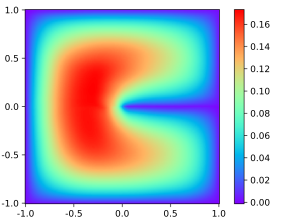
\includegraphics[width=\linewidth]{../figuras/cite/deep_ritz_a.png}
		\caption{Solução pelo \textit{Deep Ritz Method}.}
		\label{fig:deep_ritz_poisson_a}
	\end{subfigure}
	\begin{subfigure}{.49\textwidth}
		\centering
		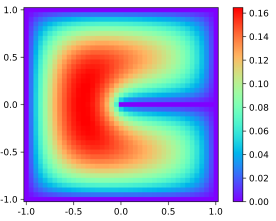
\includegraphics[width=\linewidth]{../figuras/cite/deep_ritz_b.png}
		\caption{Solução pelo método das diferenças finitas.}
		\label{fig:deep_ritz_poisson_b}
	\end{subfigure}
	\label{fig:deep_ritz_poisson}
	\legend{\ABNTEXfontereduzida Fonte: \citeonline[p. 5]{deep_ritz}.}
\end{figure}

\section{A Linguagem Python}

%{\color{red}Falar sobre a linguagem Python.}

%{\color{red}Citar alguns dos principais pacotes para programação cientifica (NumPy, SciPy, Matplotlib, Sympy).}

A linguagem de programação Python foi criada por volta de 1990 por Guido van Rossum no \textit{Stichting Mathematisch Centrum} nos Países Baixos \cite{Python_history}. Guido é o seu principal criador, porém, com o desenvolvimento \textit{open source}, a mesma apresenta colaborações de diversas pessoas (Atualmente, há cerca de mil colaboradores no repositório da linguagem no GitHub\footnote{\url{https://github.com/python/cpython/}}). Em 2001, foi criada a \textit{Python Software Foundation}, organização sem fins lucrativos, responsável por possuir a propriedade intelectual relacionada a Linguagem Python \cite{Python_history}.

As principais motivações para o uso da linguagem Python neste trabalho é o seu funcionamento simples, a facilidade de uso, grande comunidade de usuários, além do fato de ser uma linguagem de gratuita e de código aberto tornando-a, deste modo, acessível.

Além dos diversos colaboradores diretos no desenvolvimento da linguagem, existem os colaboradores indiretos que criam, por exemplo, os pacotes com funções prontas para o uso. Dentre os pacotes científicos mais conhecidos estão alguns do ecossistema \textit{SciPy}:

\begin{itemize}
	\item \textit{NumPy} é um pacote utilizado para computação científica contendo objetos para trabalhar com \textit{arrays} (arranjos em português) multidimensionais, rotinas de operações em \textit{arrays}, transformadas de Fourier, álgebra linear, estatística, dentre outras funcionalidades \cite{NumPy}.
	
	\item \textit{SciPy library} contém módulos para matemática, ciências e engenharia. As funções trazidas pela \textit{SciPy} permitem o trabalho com álgebra linear, cálculo, interpolação, manipulação de arquivos, otimização, processamento de sinais, entre outros \cite{SciPy}.
	
	\item \textit{Matplotlib} é uma biblioteca que permite plotar dados, tornando a visualização dos mesmos tão simples quanto possível \cite{Matplotlib}. Segundo \citeonline{Matplotlib}, a biblioteca possui um ambiente de estados de máquina similar ao utilizado no \textit{software} comercial MATLAB, trazendo uma experiência similar para usuários familiarizados com o MATLAB.
	
	\item \textit{SymPy} é uma biblioteca que contém classes e funções que permitem a manipulação simbólica de elementos matemáticos, isto é, os elementos matemáticos são representados de forma exata e não aproximados \cite{SymPy}. Por exemplo, ao se utilizar uma calculadora científica e fizermos algum cálculo com o número $\pi$, será apresentado no visor o cálculo utilizando uma aproximação para $\pi$. Já na matemática simbólica, $\pi$ não seria aproximado e, portanto, o número continuaria sendo representado pela letra grega. É importante perceber que, em determinados casos, a abordagem aproximada é mais eficiente e, em outros, a abordagem simbólica.
\end{itemize}

Existem outros pacotes científicos no ecossistema do \textit{SciPy} e, também, fora do ecossistema, porém, serão citados, aqui, apenas esses devido ao fato de que os seus usos são voltados para a matemática e aplicações.

A linguagem e ambos os componentes citados são desenvolvidos em código aberto de forma colaborativa. Uma das vantagens dessa forma de desenvolvimento é o rápido aperfeiçoamento de suas funcionalidades, documentação e, também, a rápida correção de bugs.

\chapter{Cálculo Variacional}
\label{cap:calc_var}

Um dos problemas pertinentes ao cálculo variacional é o de minimizar ou maximizar o funcional
\begin{equation}
	\label{eqn:cap_calc_var:int_funcional}
	I = \int_{x_1}^{x_2} f(x,y,y')dx\text{.}
\end{equation}

Minimizar o funcional \eqref{eqn:cap_calc_var:int_funcional} é o processo de encontrar uma função $y=y(x)$, satisfazendo as condições de contorno $y(x_1)=y_1$ e $y(x_2)=y_2$,  que faça com que o mesmo tenha valor mínimo. De modo análogo, maximizar o funcional é encontrar uma função $y=y(x)$, com $y(x_1)=y_1$ e $y(x_2)=y_2$, que faz a integral \eqref{eqn:cap_calc_var:int_funcional} ser um valor máximo. Minimizar ou maximizar um funcional é o mesmo que torná-lo estacionário. Assim, dizer que o funcional será estacionário é o mesmo que dizer que ele é mínimo ou máximo. Os valores $x_1$, $x_2$, $y_1$ e $y_2$ são números dados.

%{\color{red}O que é minimizar, maximizar, extremos?}

Para para encontrar a equação $y=y(x)$ procurada, são necessárias algumas ferramentas, dentre as quais a abordada neste estudo é a equação de Euler-Lagrange. Os conceitos, definições e resultados apresentados neste capítulo foram elaboradas segundo \citeonline{mefassan}, \citeonline{calcvar} e \citeonline{calcvar_campos}.

\section{Equação de Euler-Lagrange}
\label{sec:eq_euler_lagrange}

De início, é preciso demonstrar um Lema, conhecido como Lema de Lagrange, que servirá como base para a dedução da equação de Euler-Lagrange.

\begin{lema}
\label{lema:cap_calcvar_lema_1}
Sejam $x_1 < x_2$ fixos e $G(x)$ uma função contínua particular para $x_1 \leqslant x \leqslant x_2$. Se $$\int_{x_1}^{x_2} \eta (x) G(x) dx = 0$$
para cada função diferenciável $\eta (x)$ tal que $\eta (x_1)=\eta (x_2)=0$, concluímos que $G(x)=0$, para todo $x$ de modo que $x_1 \leqslant x \leqslant x_2$.

\begin{proof}
Suponha que existe $\overline{x}$ tal que $x_1\ < \overline{x} < x_2$ e $G(\overline{x})\neq 0$. Podemos supor, sem perda de generalidade, que $G(\overline{x})>0$. Como $G$ é contínua, existe uma vizinhança $\overline{x_1} \leqslant \overline{x} \leqslant \overline{x_2}$ onde $G(x)>0$ em toda a vizinhança.

É possível construir a seguinte função $\eta (x)$:
$$
\eta (x) = 
	\begin{cases}
		0 											& \mbox{para } x_1 \leqslant x < \overline{x_1}\\
		(x-\overline{x_1})^2(x-\overline{x_2})^2	& \mbox{para } \overline{x_1} \leqslant x \leqslant \overline{x_2}\\
		0											& \mbox{para } \overline{x_2} < x \leqslant x_2
	\end{cases}
$$
e então reescrever a integral do seguinte modo:
$$\int_{x_1}^{x_2}\eta (x) G(x)dx =\int_{\overline{x_1}}^{\overline{x_2}}(x-\overline{x_1})^2(x-\overline{x_2})^2G(x)dx\text{.}$$

Como $G(x) > 0$ em $\overline{x_1} \leqslant x \leqslant \overline{x_2}$, a integral do lado direito é estritamente positiva, contradizendo a hipótese. Portanto, $G(\overline{x})=0$. A demonstração considerando $G(\overline{x})<0$ é análoga.
\end{proof}
\end{lema}

Suponha $x_1$, $x_2$, $y_1$, $y_2$ dados, $f$ uma função de $x$, $y$ e $y'$ duas vezes diferenciável. É preciso construir uma família de funções admissíveis\footnote{Em outras literaturas, essas funções admissíveis podem ser chamadas, também, de funções aproximadoras, porém, devido ao uso de nomes parecidos em outros capítulos deste trabalho, foi preferível o emprego do nome funções admissíveis.}, $Y_{\varepsilon}(x)$, definida por:
\begin{equation}\label{eqn:cap_calc_var:func_admissible}
	Y_{\varepsilon}(x)=y(x)+\varepsilon \eta (x)\text{,}
\end{equation}
onde $\eta (x)$ é uma função diferenciável arbitrária para a qual $\eta (x_1)=\eta (x_2) = 0$. O número $\varepsilon$ é o parâmetro da família. A representação gráfica das funções admissíveis pode ser vista na Figura \ref{fig:funcoes_admissiveis}. Assim, a derivada de $Y$ em relação a $x$, $Y'(x)$, é
\begin{equation}\label{eqn:cap_calc_var:func_admissible_diff}
	Y'(x)=y'(x)+\varepsilon \eta '(x)\text{.}
\end{equation}

\begin{figure}[!h]
	\caption{Representação gráfica das funções admissíveis.}
	\centering
	
	\resizebox{0.75\textwidth}{!}
	{
		\begin{tikzpicture}
	\tkzInit[xmin=-1, xmax=6, ymin=-1, ymax=6]
	% draw axis without ticks
	\tkzDrawX[noticks]
	\tkzDrawY[noticks]
	
	% define extrems on y(x) curve
	\tkzDefPoint[](2.5, 2.0){A}
	\tkzDefPoint[](4.6, 3.76){B}		
	% define helper points
	\tkzDefPoint[](2.5, 0.0){C}
	\tkzDefPoint[](4.6, 0.0){D}
	\tkzDefPoint[](0.0, 2.0){E}
	\tkzDefPoint[](0.0, 3.76){F}
	% helper points to put labels
	\tkzDefPoint[](3.4, 3.2){G}
	\tkzDefPoint[](2.6, 1.7){H}
	\tkzDefPoint[](3.7, 4.2){I}
	\tkzDefPoint[](3.2, 0.4){J}
	
	% draw extrem points on y(x) curve
	\tkzDrawPoint[fill=black, size=7](A)
	\tkzDrawPoint[fill=black, size=7](B)
		
	% y(x)
	\tkzFct[domain=2.5:4.6,samples=1000, line width=2pt]{-exp(-x+3.2)+4}
	% eta(x)
	\tkzFct[domain=2.5:4.6,samples=1000]{-0.18*x*x+1.29*x-2.09}
	% y(x) + 2*eta(x)
	\tkzFct[domain=2.5:4.6,samples=1000,dashed]{-exp(-x+3.2)+4+2*(-0.18*x*x+1.29*x-2.09)}
	% y(x) - 4*eta(x)
	\tkzFct[domain=2.5:4.6,samples=1000,dashed]{-exp(-x+3.2)+4-4*(-0.18*x*x+1.29*x-2.09)}
		
	% draw dotted segments (x_1, y_1), (x_2, y_2)
	\tkzDrawSegment[dotted](A,C)
	\tkzDrawSegment[dotted](B,D)
	\tkzDrawSegment[dotted](A,E)
	\tkzDrawSegment[dotted](B,F)
		
	% x_1, x_2, y_1, y_2 labels
	\tkzLabelPoint[below](C){$x_1$}
	\tkzLabelPoint[below](D){$x_2$}
	\tkzLabelPoint[left](E){$y_1$}
	\tkzLabelPoint[left](F){$y_2$}
	
	\tkzLabelPoint[right](G){$y(x)$}
	\tkzLabelPoint[right](H){$Y_2(x)=y(x)+\varepsilon _2 \eta(x)$}
	\tkzLabelPoint[right](I){$Y_1(x)=y(x)+\varepsilon _1 \eta(x)$}
	\tkzLabelPoint[right](J){$\eta(x)$}
\end{tikzpicture}
	}
	
	\label{fig:funcoes_admissiveis}
	\legend{\ABNTEXfontereduzida Fonte: Elaborada pelo autor, 2019.}
\end{figure}

Reescrevendo a integral (\ref{eqn:cap_calc_var:int_funcional}) utilizando as funções admissíveis definidas, tem-se
\begin{equation}\label{eqn:cap_calc_var:int_funcional_approx}
I(\varepsilon)=\int_{x_1}^{x_2}f(x, Y_{\varepsilon}, Y')dx\text{.}
\end{equation}

Note que a função procurada $y(x)$ é o membro da família $Y(x)$ quando $\varepsilon = 0$. Ou seja, se $\varepsilon = 0$ pode-se substituir $Y$ e $Y'$ por $y$ e $y'$, respectivamente. Deste modo, a função que determina os extremos do funcional em \eqref{eqn:cap_calc_var:int_funcional_approx} é a mesma que determina os extremos em \eqref{eqn:cap_calc_var:int_funcional} tomando $\varepsilon=0$.

A condição necessária para que uma função de uma variável real tenha um extremo em algum ponto é que sua primeira derivada se anule nesse ponto. Então, é necessário que
\begin{equation}\label{eqn:cap_calc_var:extrem_condition}
	I'(0)=0\text{.}
\end{equation}

{\color{red}Deixar explicito que $I'(\varepsilon)$ é a derivada de $I$ em relação a $\varepsilon$ enquanto que $Y'$ ou $y'$ é a derivada de $Y$ ou $y$ em relação a $x$.}

Utilizando a Regra de Leibniz (Teorema \ref{teorema:regra_de_leibniz} do Apêndice \ref{apend:regra_de_leibniz}), a derivada de (\ref{eqn:cap_calc_var:int_funcional_approx}) pode ser escrita como
$$I'(\varepsilon)=\int_{x_1}^{x_2} \frac{\partial f}{\partial \varepsilon} (x, Y_{\varepsilon}, Y') dx \text{,}$$
e, aplicando regra da cadeia, obtêm-se
$$I'(\varepsilon)=\int_{x_1}^{x_2}\left ( \frac{\partial f}{\partial x}\frac{\partial x}{\partial \varepsilon} + \frac{\partial f}{\partial Y} \frac{\partial Y}{\partial \varepsilon} + \frac{\partial f}{\partial Y'} \frac{\partial Y'}{\partial \varepsilon} \right )dx\text{,}$$
onde o primeiro termo do integrando é nulo, dado ao fato de que $x$ independe de $\varepsilon$, portanto $\dfrac{\partial x}{\partial \varepsilon}=0$, ou seja,
\begin{equation}\label{eqn:cap_calc_var:chain_rule}
I'(\varepsilon)=\int_{x_1}^{x_2}\left ( \frac{\partial f}{\partial Y}\frac{\partial Y}{\partial \varepsilon} + \frac{\partial f}{\partial Y'}\frac{\partial Y'}{\partial \varepsilon} \right ) dx \text{.}
\end{equation}

Derivando \eqref{eqn:cap_calc_var:func_admissible} em função de $\varepsilon$, tem-se $\dfrac{\partial Y}{\partial \varepsilon}=\dfrac{\partial y}{\partial \varepsilon}+\dfrac{\partial}{\partial \varepsilon}(\varepsilon \eta)$, de onde conclui-se que $\dfrac{\partial Y}{\partial \varepsilon}=\eta$, pois $y$ e $\eta$ independem de $\varepsilon$. O mesmo acontece com \eqref{eqn:cap_calc_var:func_admissible_diff}, donde verifica-se que $\dfrac{\partial Y'}{\partial \varepsilon}=\eta'$. Deste modo, de \eqref{eqn:cap_calc_var:chain_rule}, obtêm-se a integral
$$I'(\varepsilon)=\int_{x_1}^{x_2}\left ( 
	\frac{\partial f}{\partial Y} \eta +
	\frac{\partial f}{\partial Y'} \eta '
\right )dx \text{.}
$$

Para calcular $I'(0)$, tem-se que $\varepsilon=0$ e, então, podemos trocar $Y$ e $Y'$ por $y$ e $y'$, respectivamente, obtendo
$$
I'(0)=\int_{x_1}^{x_2}\left (
	\frac{\partial f}{\partial y} \eta +
	\frac{\partial f}{\partial y'} \eta '
\right )dx
$$
$$
I'(0)=
	\int_{x_1}^{x_2} \frac{\partial f}{\partial y}\eta dx
	+
	\int_{x_1}^{x_2} \frac{\partial f}{\partial y'}\eta' dx \text{.}
$$

Integrando a segunda parcela, por partes, tomando $u=\dfrac{\partial f}{\partial y'}$ e $dv=\eta'dx$ de onde obtêm-se $du=\dfrac{d}{dx}\left ( \dfrac{\partial f}{\partial y'} \right )dx$ e $v=\eta$, segue que,
$$
I'(0)=
	\int_{x_1}^{x_2} \frac{\partial f}{\partial y}\eta dx
	+
	\left (
	uv \Big|_{x_1}^{x_2} - \int_{x_1}^{x_2}vdu
	\right )
$$
\begin{equation}\label{eqn:cap_calc_var:integration_parts}
I'(0)=
	\int_{x_1}^{x_2} \frac{\partial f}{\partial y}\eta dx
	+
	\left (
		\frac{\partial f}{\partial y'}\eta \Biggr|_{x_1}^{x_2} - \int_{x_1}^{x_2} \frac{d}{dx}\left ( \frac{\partial f}{\partial y'} \right ) \eta dx
	\right )
\end{equation}

Sabe-se que $\dfrac{\partial f}{\partial y'}\eta \Big |_{x_1}^{x_2}=0$, devido ao fato de que $\eta(x_1)=\eta(x_2)=0$, portanto, \eqref{eqn:cap_calc_var:integration_parts} pode ser reescrita como
\begin{equation}
	\label{eqn:cap_calc_var:func_admitindo_eta_0}
	I'(0)=
		\int_{x_1}^{x_2} \frac{\partial f}{\partial y}\eta dx
		-
		\int_{x_1}^{x_2} \frac{d}{dx} \left ( \frac{\partial f}{\partial y'} \right ) \eta dx
\end{equation}
$$
I'(0)=\int_{x_1}^{x_2}\left (
	\frac{\partial f}{\partial y} -
	\frac{d}{dx}
	\left (
		\frac{\partial f}{\partial y'}
	\right )
\right )\eta dx
$$
que, a partir da condição necessária (\ref{eqn:cap_calc_var:extrem_condition}), deve ser igualada a $0$:
$$
I'(0)=\int_{x_1}^{x_2}\left (
	\frac{\partial f}{\partial y} -
	\frac{d}{dx}
	\left (
		\frac{\partial f}{\partial y'}
	\right )
\right )\eta dx = 0	\text{.}
$$
permitindo, pelo Lema \ref{lema:cap_calcvar_lema_1}, obter a seguinte equação:
\begin{equation}\label{eqn:cap_calc_var:euler_lagrange}
\frac{\partial f}{\partial y} - \frac{d}{dx} \left ( \frac{\partial f}{\partial y'} \right )=0 \text{.}
\end{equation}

A equação diferencial \eqref{eqn:cap_calc_var:euler_lagrange} é chamada de equação de Euler-Lagrange e permite encontrar uma função $f$ que maximiza ou minimiza a integral (\ref{eqn:cap_calc_var:int_funcional}).

\section{Equação de Euler-Lagrange para funcionais que dependem das derivadas de ordem superior}
\label{sec:eq_euler_lagrange_superior}

Existem também, funcionais que dependem de mais funções, funções de mais de uma variável ou, ainda, que dependem de derivadas de ordem superior. O último caso será mostrado aqui, tendo em vista seu uso nos próximos capítulos. Considere o funcional
\begin{equation}
	\label{eqn:cap_calc_var:funcional_n_derivadas}
	I=\int_{x_1}^{x_2} f(x, y, y', y'', \dots, y^{(n)})dx
	\text{,}
\end{equation}
onde $y^{(n)}$ representa a $n$-ésima derivada de $y$. Pode-se aproximar $y(x)$ através de funções admissíveis $Y_{\varepsilon}(x)=y(x)+\varepsilon \eta (x)$, onde $\eta(x_1)=\eta(x_2)=0$ e $\eta(x)$ deve ser uma função de classe $C^n$, isto é, $n$ vezes diferenciável com suas derivadas contínuas. Desse modo,
$$
	Y'(x)=y'(x)+\varepsilon \eta ' (x)
	\text{,}
$$
$$
	Y''(x)=y''(x)+\varepsilon \eta '' (x)
	\text{,}
$$
$$
	\vdots
$$
$$
	Y^{(n)} (x)= y^{(n)}(x)+\varepsilon \eta^{(n)} (x)
	\text{.}
$$

Substituindo $y$, $y'$, $y''$, $\dots$, $y^{(n)}$ por suas funções admissíveis $Y$, $Y'$, $Y''$, $\dots$, $Y^{(n)}$ em \eqref{eqn:cap_calc_var:funcional_n_derivadas}, o funcional pode ser escrito como
$$
	I(\varepsilon) = \int_{x_1}^{x_2}
		f(x, Y_{\varepsilon}, Y', Y'', \dots, Y^{(n)})
		dx
	\text{,}
$$
donde, derivando em função de $\varepsilon$, por meio da Regra de Leibniz (Teorema \ref{teorema:regra_de_leibniz} do Apêndice \ref{apend:regra_de_leibniz}), tem-se
\begin{equation}
	\label{eqn:cap_calc_var:diff_func_n_derivadas_leibniz}
	I'(\varepsilon) = 
	\int_{x_1}^{x_2}
		\frac{\partial f}{\partial \varepsilon}
		(x, Y_{\varepsilon}, Y', Y'', \dots, Y^{(n)})
		dx
	\text{.}
\end{equation}

Aplicando a Regra da Cadeia em \eqref{eqn:cap_calc_var:diff_func_n_derivadas_leibniz}, $I'(\varepsilon)$ pode ser escrita como
$$
	I'(\varepsilon)=\int_{x_1}^{x_2}
	\left (
		\frac{\partial f}{\partial x}
		\frac{\partial x}{\partial \varepsilon}
		+
		\frac{\partial f}{\partial Y}
		\frac{\partial Y}{\partial \varepsilon}
		+
		\frac{\partial f}{\partial Y'}
		\frac{\partial Y'}{\partial \varepsilon}
		+
		\frac{\partial f}{\partial Y''}
		\frac{\partial Y''}{\partial \varepsilon}
		+
		\cdots
		+
		\frac{\partial f}{\partial Y^{(n)}}
		\frac{\partial Y^{(n)}}{\partial \varepsilon}
	\right ) dx
	\text{,}
$$
onde $\dfrac{\partial x}{\partial \varepsilon} = 0$, pois $x$ não depende de $\varepsilon$, assim,
\begin{equation}
	\label{eqn:cap_calc_var:func_n_derivadas_pos_regra_cadeia}
	I'(\varepsilon)=\int_{x_1}^{x_2}
	\left (
		\frac{\partial f}{\partial Y}
		\frac{\partial Y}{\partial \varepsilon}
		+
		\frac{\partial f}{\partial Y'}
		\frac{\partial Y'}{\partial \varepsilon}
		+
		\frac{\partial f}{\partial Y''}
		\frac{\partial Y''}{\partial \varepsilon}
		+
		\cdots
		+
		\frac{\partial f}{\partial Y^{(n)}}
		\frac{\partial Y^{(n)}}{\partial \varepsilon}
	\right ) dx
	\text{.}
\end{equation}

Derivando as funções admissíveis $Y$, $Y'$, $Y''$, $\dots$, $Y^{(n)}$ em relação a $\varepsilon$, como já feito anteriormente, é possível substituir em \eqref{eqn:cap_calc_var:func_n_derivadas_pos_regra_cadeia}, os valores de $\dfrac{\partial Y}{\partial \varepsilon}$ por $\eta(x)$ e $\dfrac{\partial Y^{(i)}}{\partial \varepsilon}$ por $\eta^{(i)}(x)$ onde $i=1, 2, \dots, n$. Assim, \eqref{eqn:cap_calc_var:func_n_derivadas_pos_regra_cadeia} pode ser reescrito como
\begin{equation}
	\label{eqn:cap_calc_var:func_n_derivadas_replace_0}
	I'(\varepsilon)=
	\int_{x_1}^{x_2} \left (
		\frac{\partial f}{\partial Y} \eta
		+
		\frac{\partial f}{\partial Y'} \eta'
		+
		\frac{\partial f}{\partial Y''} \eta''
		+
		\cdots
		+
		\frac{\partial f}{\partial Y^{(n)}} \eta^{(n)}
	\right ) dx
	\text{.}
\end{equation}

Fazendo $\varepsilon=0$, pode-se substituir $Y$, $Y'$, $Y''$, $\dots$, $Y^{(n)}$ por $y$, $y'$, $y''$, $\dots$, $y^{(n)}$, respectivamente, então
$$
	I'(0)= \int_{x_1}^{x_2} \left (
		\frac{\partial f}{\partial y} \eta
		+
		\frac{\partial f}{\partial y'} \eta'
		+
		\frac{\partial f}{\partial y''} \eta''
		+
		\cdots
		+
		\frac{\partial f}{\partial y^{(n)}} \eta^{(n)}
	\right )dx
$$
\begin{equation}
	\label{eqn:cap_calc_var:func_n_derivadas_pos_separar}
	I'(0)= 
	\int_{x_1}^{x_2}
		\frac{\partial f}{\partial y} \eta
	dx
	+		
	\int_{x_1}^{x_2}
		\frac{\partial f}{\partial y'} \eta'
	dx
	+
	\int_{x_1}^{x_2}
		\frac{\partial f}{\partial y''} \eta''
	dx
	+
	\cdots
	+
	\int_{x_1}^{x_2}
		\frac{\partial f}{\partial y^{(n)}} \eta^{(n)}
	dx
	\text{.}
\end{equation}

As integrações para o caso geral serão omitidas aqui. Nas duas subseções proximas, será mostrado o processo para o caso em que $n=2$ e a equação geral para derivadas até a ordem $n$.

\subsection{Processo para funcionais que dependem de derivadas de segunda ordem}

Fazendo uso de \eqref{eqn:cap_calc_var:funcional_n_derivadas} e \eqref{eqn:cap_calc_var:func_n_derivadas_pos_separar} pode-se considerar o caso em que $n=2$, onde o funcional é dado por
$$
	I=\int_{x_1}^{x_2} f(x, y, y', y'')dx
	\text{,}
$$
e $I'(0)$ é dado por
\begin{equation}
	\label{eqn:cap_calc_var:func_2_derivada_integracao}
	I'(0)=
	\int_{x_1}^{x_2}
		\frac{\partial f}{\partial y}
		\eta
	dx
	+
	\int_{x_1}^{x_2}
		\frac{\partial f}{\partial y'}
		\eta'
	dx
	+
	\int_{x_1}^{x_2}
		\frac{\partial f}{\partial y''}
		\eta''
	dx
	\text{.}
\end{equation}

A segunda parcela pode ser integrada, por partes, com $u=\dfrac{\partial f}{\partial y'}$ e $dv=\eta'dx$, donde 
$du=\dfrac{d}{dx} \left (
	\dfrac{\partial f}{\partial y'}
\right ) dx$ e $v=\eta$, logo
$$
	\int_{x_1}^{x_2} \frac{\partial f}{\partial y'}\eta ' dx
	=
	\frac{\partial f}{\partial y'}\eta \Big |_{x_1}^{x_2}
	-
	\int_{x_1}^{x_2}
		\frac{d}{dx} \left (
			\frac{\partial f}{\partial y'}
		\right ) \eta dx
	\text{,}
$$
mas $\eta(x_1)=\eta(x_2)=0$, ou seja, a integral pode ser reescrita como
\begin{equation}
	\label{eqn:cap_calc_var:func_2_derivadas_membro2}
	\int_{x_1}^{x_2} \frac{\partial f}{\partial y'}\eta ' dx
	=
	-
	\int_{x_1}^{x_2}
		\frac{d}{dx} \left (
			\frac{\partial f}{\partial y'}
		\right ) \eta dx
	\text{.}
\end{equation}

A terceira parcela deve ser integrada duas vezes por partes. Na primeira integração, seja $u=\dfrac{\partial f}{\partial y''}$ e $dv=\eta''dx$, onde 
$du=\dfrac{d}{dx} \left (
	\dfrac{\partial f}{\partial y''}
\right) dx$ e $v=\eta '$. Assim,
\begin{equation}
	\label{eqn:cap_calc_var:el_diff_2_eta2}
	\int_{x_1}^{x_2}
		\frac{\partial f}{\partial y''}
		\eta ''
	dx
	=
	\frac{\partial f}{\partial y''} \eta ' \Big |_{x_1}^{x_2}
	-
	\int_{x_1}^{x_2} \frac{d}{dx}
		\left ( 
			\frac{\partial f}{\partial y''}
		\right )
	\eta ' dx
	\text{.}
\end{equation}

Integrando, por partes, a segunda parcela de \eqref{eqn:cap_calc_var:el_diff_2_eta2}, tomando $u=\dfrac{d}{dx}\left (\dfrac{\partial f}{\partial y''}\right )$ e $dv=\eta'dx$, de onde $du=\dfrac{d^2}{dx^2}\left ( \dfrac{\partial f}{\partial y''} \right ) dx$ e $v=\eta$. Portanto,
$$
	\int_{x_1}^{x_2}
		\frac{\partial f}{\partial y''}
		\eta'' dx
	=
		\frac{\partial f}{\partial y''}\eta ' \Big |_{x_1}^{x_2}
		- \left [
		\frac{d}{dx} \left (
			\frac{\partial f}{\partial y''}
		\right ) \eta \Big |_{x_1}^{x_2}
		-
		\int_{x_1}^{x_2}
			\frac{d^2}{dx^2} \left (
				\frac{\partial f}{\partial y''}
			\right )
		\eta dx
	\right ]
	\text{,}
$$
e, como $\eta(x_1)=\eta(x_2)=0$,
\begin{equation}
	\label{eqn:cap_calc_var:el_diff_2_eta2_complete}
	\int_{x_1}^{x_2}
		\frac{\partial f}{\partial y''}
		\eta'' dx
	=
	\frac{\partial f}{\partial y''}\eta ' \Big |_{x_1}^{x_2}
	+
	\int_{x_1}^{x_2}
		\frac{d^2}{dx^2} \left (
			\frac{\partial f}{\partial y''}
		\right )
	\eta dx
	\text{.}
\end{equation}

Voltando a \eqref{eqn:cap_calc_var:func_2_derivada_integracao}, e substituindo os valores de \eqref{eqn:cap_calc_var:func_2_derivadas_membro2} e \eqref{eqn:cap_calc_var:el_diff_2_eta2_complete}, tem-se
$$
	I'(0)=
	\int_{x_1}^{x_2}
		\frac{\partial f}{\partial y}
		\eta dx
	-
	\int_{x_1}^{x_2}
		\frac{d}{dx}\left (
			\frac{\partial f}{\partial y'}
		\right ) \eta dx
	+
	\frac{\partial f}{\partial y''}\eta' \Big |_{x_1}^{x_2}
	+
	\int_{x_1}^{x_2}
		\frac{d^2}{dx^2}\left (
			\frac{\partial f}{\partial y''}
		\right ) \eta dx
	\text{,}
$$
de onde, reorganizando os termos e colocando $\eta$ em evidência, e, finalmente, fazendo $I'(0)=0$, obtem-se
\begin{equation}
	\label{eqn:cap_calc_var:cond_with_naturalbound}
	I'(0)=
	\int_{x_1}^{x_2}
	\left (
		\frac{\partial f}{\partial y}
	-
		\frac{d}{dx}\left (
			\frac{\partial f}{\partial y'}
		\right )
	+
		\frac{d^2}{dx^2}\left (
			\frac{\partial f}{\partial y''}
		\right )
	\right ) \eta dx
	+
	\frac{\partial f}{\partial y''}\eta' \Big |_{x_1}^{x_2}
	= 0
	\text{.}
\end{equation}

A segunda parcela de \eqref{eqn:cap_calc_var:cond_with_naturalbound}, $\dfrac{\partial f}{\partial y''}\eta '\Big|_{x_1}^{x_2}$ é uma das chamadas Condições de Contorno Naturais e deve-se anular para que o funcional se torne estacionário. Porém, o foco nessa parte é tratar a equação de Euler-Lagrange, que é uma condição necessária, mas não suficiente, para que o funcional se torne estacionário. As Condições de Contorno Naturais serão tratadas na seção \ref{sec:cond_contorno}. Devido, então, ao fato de que a mesma deve-se anular, resta que
\begin{equation}
	\label{eqn:cap_calc_var:func_2_derivadas_final}
	I'(0)=
	\int_{x_1}^{x_2}
	\left (
		\frac{\partial f}{\partial y}
	-
		\frac{d}{dx}\left (
			\frac{\partial f}{\partial y'}
		\right )
	+
		\frac{d^2}{dx^2}\left (
			\frac{\partial f}{\partial y''}
		\right )
	\right ) \eta dx
	\text{,}
\end{equation}
onde, utilizando o Lema \ref{lema:cap_calcvar_lema_1} em \eqref{eqn:cap_calc_var:func_2_derivadas_final}, a equação de Euler-Lagrange obtida é

\begin{equation}
	\label{eqn:cap_calc_var:eq_euler_lagrange_twodiff}
	\frac{\partial f}{\partial y}
	-
	\frac{d}{dx}\left (
		\frac{\partial f}{\partial y'}
	\right )
	+
	\frac{d^2}{dx^2}\left (
		\frac{\partial f}{\partial y''}
	\right )
	=0 \text{.}
\end{equation}

É importante ressaltar, novamente, que a equação de Euler-Lagrange \eqref{eqn:cap_calc_var:eq_euler_lagrange_twodiff} obtida é uma condição necessária, porém não é condição suficiente para a estacionáriedade do funcional.

%{\color{red}Condições de contorno......, $\dfrac{\partial f}{\partial y''}\eta ' \Big |_{x_1}^{x_2} = 0$, portanto
%$$
%	\int_{x_1}^{x_2}
%		\frac{\partial f}{\partial y''}
%		\eta'' dx
%	=
%	-
%	\int_{x_1}^{x_2}
%		\frac{d}{dx} \left (
%			\frac{\partial f}{\partial y''}
%		\right )
%	\eta 'dx
%	\text{,}
%$$}
%e, para a segunda integração por partes, pode-se fazer
%$u=\dfrac{d}{dx} \left (
%	\dfrac{\partial f}{\partial y''}
%\right )$ e $dv=\eta ' dx$, de onde 
%$du=\dfrac{d^2}{dx^2} \left (
%	\dfrac{\partial f}{\partial y''}
%\right )dx$ e $v=\eta$.  Assim,
%
%$$
%	\int_{x_1}^{x_2}
%		\frac{\partial f}{\partial y''}
%		\eta'' dx
%	=
%	- \left [
%		\frac{d}{dx} \left (
%			\frac{\partial f}{\partial y''}
%		\right ) \eta \Big |_{x_1}^{x_2}
%		-
%		\int_{x_1}^{x_2}
%			\frac{d^2}{dx^2} \left (
%				\frac{\partial f}{\partial y''}
%			\right )
%		\eta dx
%	\right ]
%	\text{,}
%$$
%e, como $\eta(x_1)=\eta(x_2)=0$,
%\begin{equation}
%	\label{eqn:cap_calc_var:func_2_derivadas_membro3}
%	\int_{x_1}^{x_2}
%		\frac{\partial f}{\partial y''}
%		\eta'' dx
%	=
%	\int_{x_1}^{x_2}
%		\frac{d^2}{dx^2} \left (
%			\frac{\partial f}{\partial y''}
%		\right )
%	\eta dx
%	\text{.}
%\end{equation}
%
%Voltando a \eqref{eqn:cap_calc_var:func_2_derivada_integracao}, substituindo os resultados de \eqref{eqn:cap_calc_var:func_2_derivadas_membro2} e \eqref{eqn:cap_calc_var:func_2_derivadas_membro3}, $I'(0)$ pode ser escrito como
%$$
%	I'(0)=
%	\int_{x_1}^{x_2}
%		\frac{\partial f}{\partial y}
%		\eta dx
%	-
%	\int_{x_1}^{x_2}
%		\frac{d}{dx}\left (
%			\frac{\partial f}{\partial y'}
%		\right ) \eta dx
%	+
%	\int_{x_1}^{x_2}
%		\frac{d^2}{dx^2}\left (
%			\frac{\partial f}{\partial y''}
%		\right ) \eta dx
%$$
%$$
%	I'(0)=
%	\int_{x_1}^{x_2} \left (
%		\frac{\partial f}{\partial y}
%		\eta
%		-
%		\frac{d}{dx}\left (
%			\frac{\partial f}{\partial y'}
%		\right ) \eta
%		+
%		\frac{d^2}{dx^2}\left (
%			\frac{\partial f}{\partial y''}
%		\right ) \eta 
%	\right ) dx
%$$
%\begin{equation}
%	\label{eqn:cap_calc_var:func_2_derivadas_final}
%	I'(0)=
%	\int_{x_1}^{x_2} \left (
%		\frac{\partial f}{\partial y}
%		-
%		\frac{d}{dx}\left (
%			\frac{\partial f}{\partial y'}
%		\right )
%		+
%		\frac{d^2}{dx^2}\left (
%			\frac{\partial f}{\partial y''}
%		\right )
%	\right ) \eta dx
%	\text{.}
%\end{equation}
%
%Fazendo $I'(0)=0$ e utilizando o Lema \ref{lema:cap_calcvar_lema_1} em \eqref{eqn:cap_calc_var:func_2_derivadas_final}, a equação de Euler-Lagrange é obtida como
%$$
%	\frac{\partial f}{\partial y}
%	-
%	\frac{d}{dx}\left (
%		\frac{\partial f}{\partial y'}
%	\right )
%	+
%	\frac{d^2}{dx^2}\left (
%		\frac{\partial f}{\partial y''}
%	\right )
%	=0 \text{.}
%$$

\subsection{Equação Geral}

%Para funcionais que dependem de derivadas superiores até a ordem $n$, o processo para obtenção da equação é análogo e a equação de Euler-Lagrange é dada por


Para a obtenção da Equação Geral, para funcionais que dependem de derivadas até a ordem $n$, o processo para a obtenção da equação de Euler-Lagrange é análogo. Em \eqref{eqn:cap_calc_var:func_n_derivadas_pos_separar} deve-se integrar a segunda parcela por partes uma vez, a terceira parcela duas vezes, a quarta parcela três vezes e assim por diante, até que a $n$-ésima parcela seja integrada $n-1$ vezes, também por partes. Ao fim do processo, a equação de Euler-Lagrange será obtida fazendo $I'(0)=0$, isto é, aplicando a condição de estacionariedade e, por último, utilizando o Lema \ref{lema:cap_calcvar_lema_1}. Deste modo, a equação encontrada é

\begin{equation}
	\label{eqn:cap_calc_var:euler_lagrange_nesimo}
	\frac{\partial f}{\partial y}
	- \frac{d}{dx}\left ( \frac{\partial f}{\partial y'} \right )
	+ \frac{d^2}{dx^2}\left ( \frac{\partial f}{\partial y''} \right )
	- \frac{d^3}{dx^3}\left ( \frac{\partial f}{\partial y'''} \right )
	+ \cdots
	+ (-1)^n \frac{d^n}{dx^n}\left (\frac{\partial f}{\partial y^{(n)}} \right )
	= 0
	\text{.}
\end{equation}

A equação \eqref{eqn:cap_calc_var:euler_lagrange_nesimo} é escrita, também, como
$$
	\sum_{i=0}^n (-1)^i\frac{d^i}{dx^i}\left (
		\frac{\partial f}{\partial y^{(i)}}
	\right )
	= 0
	\text{,}
$$
onde a primeira parcela $\dfrac{d^0}{dx^0} \left ( \dfrac{\partial f}{\partial y^0} \right )$ representa $\dfrac{\partial f}{\partial y}$.

\section{Condições de Contorno Naturais e Essenciais}
\label{sec:cond_contorno}

Durante o processo para a obtenção da função $y(x)$ que torna o funcional estacionário aparecem algumas condições de contorno que devem ser tratadas cuidadosamente. Por exemplo, tomando o funcional
$$
	I=\int_{x_1}^{x_2} f(x, y, y')dx
	\text{,}
$$
tem-se, da Seção \ref{sec:eq_euler_lagrange}, que sua condição de estacionáriedade é dada por
\begin{equation}
	\label{eqn:cap_calc_var:cond_boundary}
	\int_{x_1}^{x_2} \left (
		\frac{\partial f}{\partial y}
		-
		\frac{d}{dx} \left (
			\frac{\partial f}{\partial y'}
		\right )
	\right ) \eta dx
	+
	\frac{\partial f}{\partial y'}\eta \Big |_{x_1}^{x_2} = 0
	\text{,}
\end{equation}
onde, como já tratado, $\eta$ representa uma variação da função exata conhecida.

Admitimos, em \eqref{eqn:cap_calc_var:func_admitindo_eta_0}, que $\eta(x_1)=\eta(x_2)=0$, porém isso nem sempre acontece. Existem casos em que, para que a condição de estacionáriedade \eqref{eqn:cap_calc_var:cond_boundary} seja válida é preciso, primeiro, que a primeira parcela de \eqref{eqn:cap_calc_var:cond_boundary} seja nula, donde se resulta a equação de Euler-Lagrange
$$
	\frac{\partial f}{\partial y}
	-
	\frac{d}{dx}\left (
		\frac{\partial f}{\partial y'}
	\right )
	= 0
	\text{,}
$$
e, ainda, que
$$
	\frac{\partial f}{\partial y'}\eta \Big |_{x_1}^{x_2} = 0
	\text{,}
$$
de onde, geralmente, surgem as duas igualdades
\begin{equation}
	\label{eqn:cap_calc_var:condicao_natural_d1}
	\frac{\partial f}{\partial y'} \Big |_{x=x_1} = 0
	\text{,}
\end{equation}
\begin{equation}
	\label{eqn:cap_calc_var:condicao_natural_d2}
	\frac{\partial f}{\partial y'} \Big |_{x=x_2} = 0
	\text{.}
\end{equation}

É importante deixar claro que pode acontecer, por exemplo, de $\eta(x_1)=0$ e $\eta(x_2)\neq 0$, ou vice-versa, e, consequentemente, reduz-se uma dessas condições de contorno.

Essas condições de contorno são denominadas condições de contorno naturais do problema ou, ainda, problema de valor de contorno de Neumann. Elas tendem a aparecer normalmente durante o processo de encontrar $y(x)$ tornando o funcional estacionário.

Para o caso de funcionais que dependem de derivadas de ordem superior, da forma
$$
	I=\int_{x_1}^{x_2} f(x, y, y', \dots, y^{(n)}) dx
	\text{,}
$$
aparecem diversas condições de contorno parecidas com \eqref{eqn:cap_calc_var:condicao_natural_d1} e \eqref{eqn:cap_calc_var:condicao_natural_d2}. Um destes exemplos aparece em \eqref{eqn:cap_calc_var:cond_with_naturalbound}.

Outro tipo de condições de contorno que aparecem com problemas do Cálculo Variacional são condições de contorno geométricas. As condições de contorno geométricas precisam, necessariamente serem satisfeitas e são denominadas de condições de contorno essenciais ou, ainda, problemas de valor de contorno de Dirichlet.

\begin{exemplo}
	Considere o funcional
	\begin{equation}
		\label{eqn:cap_calc_var:funcional_pi}
		I = \frac{1}{2}	\int_{0}^{l}
			EI \left (
				\frac{d^2v}{dx^2}
			\right )^2 dx
			-
			\int_{0}^{l} qv dx
			\text{.}
	\end{equation}
	
	Variando $v$ por $\overline{v}_{\varepsilon}=v+\varepsilon \eta$ em \eqref{eqn:cap_calc_var:funcional_pi}, tem-se
	$$
		I(\varepsilon) = \frac{1}{2} \int_{0}^{l}
			EI \left (
				\frac{d^2\overline{v}}{dx^2}
			\right )^2 dx
			-
			\int_{0}^{l} q\overline{v} dx
			\text{,}
	$$
	de onde, derivando $I(\varepsilon)$ em relação a $\varepsilon$, resulta em
	\begin{equation}
		\label{eqn:cap_calc_var:natural_conditions_deduce}
		\frac{dI}{d\varepsilon} = 
			\int_{0}^{l} EI \left (
				\frac{d^2\overline{v}}{dx^2}
			\right ) \cdot 
			\frac{d}{d\varepsilon}\left (
				\frac{d^2\overline{v}}{dx^2}
			\right ) dx
			-
			\int_{0}^{l} q\frac{d\overline{v}}{d\varepsilon} dx
			\text{.}
	\end{equation}
	
	Manipulando \eqref{eqn:cap_calc_var:natural_conditions_deduce}, e calculando $I'(0)$, pois $\overline{v}$ pode ser substituido por $v$, naturalmente, chega-se a
	$$
		I'(0) = 
			\int_{0}^{l} EI \left (
				\frac{d^2v}{dx^2}
			\right ) \left (
				\frac{d^2\eta}{dx^2}
			\right ) dx
			-
			\int_{0}^{l}q\eta dx
		\text{,}
	$$
	onde a primeira parcela deve ser integrada, por partes, duas vezes, resultando em
	\begin{equation}
		\label{eqn:cap_calc_var:natural_conditions_I0}
		I'(0) = 
			\int_{0}^{l} \left (
				EI\frac{d^4 v}{dx^4}-q 
			\right ) \eta dx
			+
			EI\frac{d^2 v}{dx^2} \eta' \Big |_{0}^{l}
			-
			EI\frac{d^3 v}{dx^3} \eta \Big |_{0}^{l}
			\text{.}
	\end{equation}
	
	Aplicando a condição de estacionáriedade, $I'(0)=0$, em \eqref{eqn:cap_calc_var:natural_conditions_I0},
	\begin{equation}
		\label{eqn:cap_calc_var:natural_conditions_I0_eq_0}
		I'(0) = 
			\int_{0}^{l} \left (
				EI\frac{d^4 v}{dx^4}-q 
			\right ) \eta dx
			+
			EI\frac{d^2 v}{dx^2} \eta ' \Big |_{0}^{l}
			-
			EI\frac{d^3 v}{dx^3} \eta \Big |_{0}^{l}
			= 0
			\text{.}
	\end{equation}
	
	É preciso, então, que os termos de \eqref{eqn:cap_calc_var:natural_conditions_I0_eq_0} se anulem. A primeira parcela de \eqref{eqn:cap_calc_var:natural_conditions_I0_eq_0} resulta na equação de Euler-Lagrange
	\begin{equation}
		\label{eqn:cap_calc_var:natural_eq_euler_lagr}
		EI\frac{d^4v}{dx^4} - q = 0
		\text{,}
	\end{equation}
	enquanto que as duas outras parcelas são as condições de contorno naturais do problema
	\begin{equation}
		\label{eqn:cap_calc_var:natural_cond1}
		\frac{d^2 v}{dx^2}\Big |_{0}^{l} = 0
		\text{,}
	\end{equation}
	\begin{equation}
		\label{eqn:cap_calc_var:natural_cond2}
		\frac{d^3 v}{dx^3}\Big |_{0}^{l} = 0
		\text{.}
	\end{equation}
	
	A equação de Euler-Lagrange \eqref{eqn:cap_calc_var:natural_eq_euler_lagr} pode ser facilmente resolvida, isolando $\dfrac{d^4 v}{dx^4}$ e integrando ambos os lados da equação quatro vezes seguidas. Ao final desse processo, a função $v$ encontrada será
	\begin{equation}
		\label{eqn:cap_calc_var:natural_funcao_v}
		v(x)=\frac{q}{24EI}x^4 + \frac{C_1}{6}x^3 + \frac{C_2}{2}x^2 + C_3x + C_4
		\text{,}
	\end{equation}
	onde os coeficientes $C_1$, $C_2$, $C_3$ e $C_4$ podem ser determinados através do uso das condições de contorno naturais e essenciais.
	
	Da condição de contorno essencial, $v(0)=0$, resulta que o coeficiente $C_4=0$. Aplicando, então as condições de contorno naturais \eqref{eqn:cap_calc_var:natural_cond1}, tem-se
	$$
		\left (
			\frac{q}{2EI}x^2 + C_1x + C_2
		\right ) \Big |_{x=0}
		= 0
		\text{,}
	$$
	resultando no valor do coeficiente $C_2=0$. Utilizando o outro extremo de \eqref{eqn:cap_calc_var:natural_cond1}, tem-se
	$$
		\left (
			\frac{q}{2EI}x^2 + C_1x + C_2
		\right ) \Big |_{x=l}
		=0
		\text{,}
	$$
	onde
	$$
		\frac{ql^2}{2EI}+C_1l=0
		\text{,}
	$$
	resultando em $C_1=-\dfrac{ql}{2EI}$.
	
	Para o último coeficiente, $C_3$, será utilizado a outra condição de contorno essencial, $v(l)=0$,
	$$
		\frac{q}{24EI}l^4
		-
		\frac{ql^4}{12EI}
		+
		C_3l
		= 0
		\text{,}
	$$
	tendo, assim, como resultado, $C_3=\dfrac{ql^3}{24EI}$.
	
	Substituindo, então, os coeficientes $C_1$, $C_2$, $C_3$ e $C_4$ determinados na função $v(x)$, encontrada em \eqref{eqn:cap_calc_var:natural_funcao_v},
	$$
		v(x) = 
			\frac{q}{24EI} x^4
			-
			\frac{ql}{12EI} x^3
			+
			\frac{ql^3}{24EI} x
			\text{.}
	$$
\end{exemplo}

%{\color{red}Durante o processo para a obtenção da equação de Euler-Lagrange, (...)}

%Durante o processo para a obtenção dos extremos de um funcional, donde se deduz a equação de Euler-Lagrange, como nas seções \ref{sec:eq_euler_lagrange} e \ref{sec:eq_euler_lagrange_superior}, surgem algumas condições de contorno, como, por exemplo, o termo
%$$
%	\frac{\partial f}{\partial y'}\eta \Big |_{x_1}^{x_2}
%	=0
%$$
%na equação \eqref{eqn:cap_calc_var:integration_parts}.

%Durante o processo de encontrar um extremo para um funcional, surgem algumas condições de contorno... {\color{red}(Escrever sobre).}

\chapter{Método de Rayleigh-Ritz}
\label{cap:mrr}

Um dos objetivos do Cálculo Variacional é encontrar uma função $y(x)$ que, dentre as funções admissíveis torna o funcional estacionário. Uma das formas para se encontrar a função $y(x)$ é encontrando a Equação de Euler-Lagrange associada ao problema e, então, resolvê-la. 

A resolução de equações diferenciais e a determinação da solução exata por meio das condições de contorno do problema é, entretanto,  uma tarefa trabalhosa e, em muitos casos, até não factível. Para se esquivar de problemas como esses, surgem alguns métodos, dentre os quais está o Método de Rayleigh-Ritz.

As explicações e os conceitos aqui utilizados foram elaboradas tomando como referências os autores \citeonline{mefassan} e \citeonline{MRR_Deflex}.

O método de Rayleigh-Ritz propõe que a função $y(x)$, exata, seja substituida por uma função aproximada $v(x)$ que é formada pela combinação linear de funções $\phi _i(x)$. Uma das vantagens do uso do método é que ele não requer que as condições de contorno naturais sejam satisfeitas \cite{GROSSI_2001}. Deste modo, o método é empregado principalmente em problemas onde as condições de contorno naturais são de difícil resolução.

Considerando o funcional
$$
	I=\int_{x_1}^{x_2} f(x,y,y',\dots,y^{(m)})dx
	\text{,}
$$
com as condições de contorno $y(x_1)=y(x_2)=0$, então a função $y(x)$ é aproximada por meio da função $v(x)$ definida como
$$
	v(x) = \sum_{i=1}^n a_i \phi _i (x)
	\text{,}
$$
onde as funções $\phi_i(x)$ são chamadas de funções de forma e devem ser linearmente independente. {\color{red}Falar sobre a diferenciabilidade das $\phi_i(x)$.} Os coeficientes $a_i$ são chamados de parâmetros de deslocamento e $v(x)$ é chamada de função aproximadora.

Substituindo $y$ por $v$ no funcional, $I$ passa a ser uma função de $a_1$, $a_2$, $\dots$, $a_n$, isto é, $I=I(a_1, a_2, \dots, a_n)$. A condição de máximo ou mínimo para o funcional $I$ é, então, que as suas derivadas parciais em relação a $a_1$, $a_2$, $\dots$, $a_n$ se anulem, então
$$
	\frac{\partial I}{\partial a_i} = 0
	\text{,}
$$
com $i=1, 2, 3, \dots, n$.

\begin{exemplo}
	\label{ex:mrr_ex_livro}
	\begin{figure}[h]
		\caption{Viga prismática.}
		\centering
		\begin{tikzpicture}
			\tkzInit[xmin=-0, xmax=6, ymin=-0.6, ymax=2]
			% draw axis without ticks
			\tkzDrawX[label=$x$, noticks, loosely dashed]
			\tkzDrawY[label=$v(x)$, noticks]
			
			% rectangle
			\tkzDefPoints{
				0/0.6/V_1,
				5/0.6/V_2,
				5/-0.6/V_3,
				0/-0.6/V_4}
			% complete x axis without dashed line
			\tkzDefPoints{
				5/0/A_1,
				6.35/0/A_2}
			% left base triangle
			\tkzDefPoints{
				0/-0.6/T1_1, 
				-0.25/-1.1/T1_2, 
				0.25/-1.1/T1_3}
			% right base triangle
			\tkzDefPoints{
				5/-0.6/T2_1, 
				4.75/-1.1/T2_2,
				5.25/-1.1/T2_3}
			% line on base of right triangle
			\tkzDefPoints{
				4.75/-1.2/T2_B1,
				5.25/-1.2/T2_B2}
			% length marker in bottom
			\tkzDefPoints{
				0/-1.5/L_1,
				0/-2/L_2,
				5/-1.5/L_3,
				5/-2/L_4,
				0/-1.75/LS_1,
				5/-1.75/LS_2}
			
			\tkzDrawSegment[color=black, line width=0.5mm](A_1, A_2)
			
			\tkzDrawPolygon[draw=black](T1_1, T1_2, T1_3)
			\tkzDrawPolygon[draw=black](T2_1, T2_2, T2_3)
			\tkzDrawSegment[color=black](T2_B1, T2_B2)
			\tkzDrawPolygon[draw=black](V_1, V_2, V_3, V_4)
			% q arrows
			\foreach \i in {1,...,25}{
				\tkzDefPoint(0.2*\i,1.3){A_\i}
				\tkzDefPoint(0.2*\i,0.7){B_\i}
				\draw[line width=0.6pt, black,-stealth] (A_\i) -- (B_\i);
			}
			% q text
			\node at (2.5,1.7) {$q$};
			% length marker in bottom
			\tkzDrawSegment[color=black](L_1, L_2)
			\tkzDrawSegment[color=black](L_3, L_4)
			\tkzDrawSegment[color=black](LS_1, LS_2)
			\node at (2.5,-2) {$l$};
		\end{tikzpicture}
		\label{fig:test_02}
		\legend{\ABNTEXfontereduzida Fonte: Elaborada pelo autor, 2019.}
	\end{figure}
	
	A viga prismática da Figura \ref{fig:test_02} possui o funcional de energia potencial total associado
	\begin{equation}
		\label{eqn:cap_metodo_ray_ritz:exemplo_func_pi}
		\Pi = 
		\frac{1}{2} \int_0^l EI \left [
			\frac{d^2v}{dx^2}
		\right ]^2 dx
		-
		\int_0^l qvdx
		\text{,}
	\end{equation}
	onde $E$ é o módulo de Young do material e I é o momento de inércia da seção transversal da viga em relação ao eixo baricêntrico. É possível encontrar uma função $v(x)$ que aproxime a função exata $y(x)$ tornando o funcional \eqref{eqn:cap_metodo_ray_ritz:exemplo_func_pi} estacionário utilizando o método de Rayleigh-Ritz. Esse processo será feito utilizando três funções aproximadoras $v(x)$:
	\begin{equation}
		\label{eqn:cap_metodo_ray_ritz_funcdef_v1}
		v_1 (x) = a_0 + a_1 x + a_2 x^2
		\text{,}
	\end{equation}
	\begin{equation}
		\label{eqn:cap_metodo_ray_ritz_funcdef_v2}
		v_2 (x) = a_0 + a_1 x + a_2 x^2 + a_3 x^3
		\text{,}
	\end{equation}
	\begin{equation}
		\label{eqn:cap_metodo_ray_ritz_funcdef_v3}
		v_3 (x) = a_0 + a_1 x + a_2 x^2 + a_3 x^3 + a_4 x^4
		\text{.}
	\end{equation}
	
	\citeonline{mefassan} cita que o ponto $y(\frac{l}{2})$ é o valor de máxima deflexão da Viga da Figura \ref{fig:test_02}. Esse valor, encontrado analiticamente, é
	\begin{equation}
		\label{eqn:cap_metodo_ray_ritz:ex1_max_deflex_exato}
		y(\frac{l}{2})=\frac{5ql^4}{384EI}
		\text{,}
	\end{equation}
	e será utilizado como parâmetro de comparação para os resultados com as funções $v_1(x)$, $v_2(x)$ e $v_3(x)$ definidas em \eqref{eqn:cap_metodo_ray_ritz_funcdef_v1}, \eqref{eqn:cap_metodo_ray_ritz_funcdef_v2} e \eqref{eqn:cap_metodo_ray_ritz_funcdef_v3}.
	
	Como primeira aproximação, pode-se utilizar a função $v_1(x)=a_0+a_1x+a_2x^2$, de onde, considerando as condições de contorno essenciais, tem-se que $v_1(0)=0$, levando a $a_0=0$, e de $v_1(l)=0$, concluindo que $a_1=-a_2l$. Assim, a função é escrita como
	$$
		v_1(x)=a_2(x^2-lx)
		\text{.}
	$$
	
	Sua derivada é $v_1'(x)=a_2(2x-l)$ e, a derivada de segunda ordem é $v_1''(x)=2a_2$. Substituindo esses valores no funcional \eqref{eqn:cap_metodo_ray_ritz:exemplo_func_pi}, tem-se que
	$$
		\Pi =
		\frac{1}{2}
		\int_0^l 4 EI a_2 ^2 dx
		-
		\int_0^l q a_2 (x^2-lx) dx
		\text{.}
	$$
	
	Da condição de estacionáriedade tem-se, que $\dfrac{\partial \Pi}{\partial a_2} = 0$ e, consequentemente
	$$
		\frac{\partial \Pi}{\partial a_2}
		=
		\frac{\partial}{\partial a_2} \left [
			\int_0^l \left ( 2EIa_2 ^2 - a_2 q (x^2 -lx) \right ) dx
		\right]
		= 0
	$$
	$$
		\frac{\partial \Pi}{\partial a_2}
		=
		\int_0^l
			\frac{\partial}{\partial a_2} \left [
			4EIa_2^2 - a_2 q(x^2-lx)
		\right ] dx
		= 0
	$$
	$$
		\frac{\partial \Pi}{\partial a_2}
		=
		\int_0^l \left [
			4EIa_2 - q(x^2-lx)
		\right ] dx
		= 0
	$$
	$$
		\left [ 
			4EIa_2 x \Big |_0^l
			-
			q \left (
				\frac{x^3}{3} - \frac{lx^2}{2}
			\right ) \Big |_0^l
		\right ] 
		= 0
	$$
	$$
		4EIa_2l
		-
		q \left (\frac{l^3}{3} - \frac{l^3}{2} \right )
		= 0
	$$	
	$$
		4EIa_2l+\frac{ql^3}{6} = 0
	$$
	$$
		a_2=\frac{-ql^2}{24EI}\text{.}
	$$

	Com o valor de $a_2$ conhecido, é possível determinar o valor de $a_1=-a_2l$, resultando em
	$$
		a_1=\frac{ql^3}{24EI}
		\text{.}
	$$
	
	Assim, a função aproximadora $v_1$ pode ser escrita como
	$$
		v_1(x)=
		\frac{ql^3}{24EI}x
		-
		\frac{ql^2}{24EI}x^2
		\text{.}
	$$
	
	Calculando $v(\frac{l}{2})$ a título de comparação com o valor exato de máxima deflexão da viga, dado por \eqref{eqn:cap_metodo_ray_ritz:ex1_max_deflex_exato},
	\begin{equation}
		\label{eqn:cap_metodo_ray_ritz:ex1_max_deflex_apv1}
		v_3(\frac{l}{2}) = \frac{ql^4}{96EI}
		\text{.}
	\end{equation}
	
	Note que há uma grande diferença entre o valor encontrado pela função $v_1(x)$, \eqref{eqn:cap_metodo_ray_ritz:ex1_max_deflex_apv1}, e o valor exato, \eqref{eqn:cap_metodo_ray_ritz:ex1_max_deflex_exato}. Visando uma melhoria nessa aproximação, faz-se necessário o uso da função definida $v_2(x)=a_0+a_1x+a_2x^2+a_3x^3$. Das condições de contorno essenciais, $v_2(0)=0$, de onde $a_0=0$, e $v_2(l)=0$, isolando $a_1=-a_2 l - a_3 l^2$. Assim, a função $v_2(x)$ é
	\begin{equation}
		\label{eqn:cap_metodo_ray_ritz:v2_organizada}
		v_2(x)=
		a_2(x^2-lx)
		+
		a_3(x^3-l^2x)
		\text{.}
	\end{equation}
	
	Derivando a função $v_2$ em função de x, duas vezes, pode-se obter
	$$
	v_2'(x) = a_2(2x-l) + a_3(3x^2-l^2)
	$$

	\begin{equation}
		\label{eqn:cap_metodo_ray_ritz:v2_diff_organizada}
		v_2''(x) = 2a_2 + 6a_3 x \text{.}
	\end{equation}
	
	Substituindo \eqref{eqn:cap_metodo_ray_ritz:v2_organizada} e \eqref{eqn:cap_metodo_ray_ritz:v2_diff_organizada} em $\Pi$, tem-se
	$$
		\Pi=
		\frac{1}{2}
		\int_0^l
			\left (
				EI(2a_2+6a_3x)^2
			\right ) dx
		-
		\int_0^l
			q
			\left (
				a_2(x^2-lx)
				+
				a_3(x^3-l^2x)
			\right ) dx
		\text{.}
	$$
	
	Derivando $\Pi$ em função de $a_2$ é possível obter
	$$
		\frac{\partial \Pi}{\partial a_2}
		=
		\int_0^l \left [
			2EI(2a_2+6a_3x)-q(x^2-lx)
		\right ] dx
		= 0
	$$	
	$$
		\frac{\partial \Pi}{\partial a_2}
		=
		\int_0^l \left [
			EI(4a_2+12a_3x)-q(x^2-lx)
		\right ] dx
		= 0
	$$
	$$
		\int_0^l \left [
			4EIa_2 + 12EIa_3x - qx^2 + qlx
		\right ] dx
		= 0
	$$
	$$
		4EIa_2 x \Big |_0^l
		+
		\frac{12a_3EI}{2} x^2 \Big |_0^l
		-
		\frac{q}{3} x^3 \Big |_0^l
		+
		\frac{ql}{2} x^2 \Big |_0^l
		= 0
	$$
	$$
		4EIa_2l
		+
		6a_3EIl^2
		-
		\frac{2ql^3}{6}
		+
		\frac{3ql^3}{6}
		= 0
	$$
	$$
		4EIa_2l
		+
		6a_3EIl^2
		=
		\frac{2ql^3}{6}
		-
		\frac{3ql^3}{6}
	$$
	$$
		4a_2 + 6a_3l
		=
		\frac{-ql^2}{6EI}
	$$
	\begin{equation}
		\label{eq:exemp_rayritz_approx2_eq1}
		2a_2 + 3a_3l
		=
		\frac{-ql^2}{12EI}
		\text{.}
	\end{equation}
	
	Derivando $\Pi$ em relação a $a_3$ tem-se que
	$$
		\frac{\partial \Pi}{\partial a_3}
		=
		\int_0^l \left [
			6EI(2a_2 + 6a_3x)x
			-
			q(x^3 - l^2x)
		\right ] dx
		= 0
	$$
	$$
		\int_0^l \left [
			EI(12a_2 + 36a_3x)x
			-
			q(x^3 - l^2x)
		\right ] dx
		= 0
	$$
	$$
		\int_0^l \left [
			EI(12a_2 x + 36a_3x^2)
			-
			q(x^3 - l^2x)
		\right ] dx = 0
		= 0
	$$
	$$
		EI \left (
			\frac{12a_2}{2}x^2 \Big |_0^l
			+
			\frac{36a_3}{3}x^3 \Big |_0^l
		\right )
		-
		q \left (
			\frac{x^4}{4} \Big |_0^l
			-
			\frac{l^2x^2}{2} \Big |_0^l
		\right )
		= 0
	$$
	$$
		EI(6a_2l^2 + 12a_3l^3)
		-
		q \left (
			\frac{l^4}{4}
		\right )
		+
		q \left (
			\frac{l^4}{2}
		\right )
	$$
	$$
		6a_2 + 12a_3l = -\frac{ql^4}{4EIl^2}
	$$
	$$
		6a_2 + 12a_3l = -\frac{ql^2}{4EI}
	$$
	\begin{equation}
		\label{eq:exemp_rayritz_approx2_eq2}
		2a_2 + 4a_3l = -\frac{ql^2}{12EI}
		\text{.}
	\end{equation}
	
	Montando um sistema de equações com \eqref{eq:exemp_rayritz_approx2_eq1} e \eqref{eq:exemp_rayritz_approx2_eq2} é possível encontrar os valores de $a_2$ e $a_3$. Fazendo \eqref{eq:exemp_rayritz_approx2_eq2} - \eqref{eq:exemp_rayritz_approx2_eq1}, tem-se $2a_2+4a_3l-2a_2-3a_3l=-\dfrac{ql^2}{12EI}+\dfrac{ql^2}{12EI}$, donde $a_3l=0$ e, então, $a_3=0$. De volta a \eqref{eq:exemp_rayritz_approx2_eq1}, substituindo $a_3=0$, reduzimos a equação a $2a_2=-\dfrac{ql^2}{12EI}$ e, por fim,
	$$
		a_2=-\frac{ql^2}{24EI}
		\text{.}
	$$

	Assim, a função $v_2(x)$ é a mesma que $v_1(x)$, não permitindo uma melhoria na aproximação desejada, sendo, portanto, inútil para esse caso. Ainda, visando melhor aproximação, deve-se passar para a próxima função aproximadora escolhida, $v_3(x)$.
	
	Utilizando a função $v_3(x)=a_0+a_1x+a_2x^2+a_3x^3+a_4x^4$, tem-se das condições de contorno essensiais que $v_3(0)=0$, donde $a_0=0$ e, $v_3(l)=0$, isto é $a_1l+a_2l^2+a_3l^3+a_4l^4=0$, donde pode-se concluir que $a_1=-a_2l-a_3l^2-a_4l^3$. Substituindo $a_0$ e $a_1$ em $v_3(x)$, podemos encontrar a função
	\begin{equation}
		\label{eqn:cap_metodo_ray_ritz:func_def_v3}
		v_3(x)=
		a_2 (x^2 - lx)
		+
		a_3 (x^3 - l^2x)
		+
		a_4 (x^4 - l^3x)
		\text{.}
	\end{equation}
	
	Derivando $v_3$ em relação a $x$, duas vezes:
	$$
		v_3'(x)=
		a_2(2x - l)
		+
		a_3(3x^2 - l^2)
		+
		a_4(4x^3 - l^3)
	$$
	\begin{equation}
		\label{eqn:cap_metodo_ray_ritz:func_def_v3_diff}
		v_3''(x)=
		2a_2
		+
		6a_3 x
		+
		12a_4 x^2
		\text{.}
	\end{equation}
	
	Substituindo \eqref{eqn:cap_metodo_ray_ritz:func_def_v3} e \eqref{eqn:cap_metodo_ray_ritz:func_def_v3_diff} em $\Pi$,
	$$
		\Pi = \frac{1}{2} \int_0^l \left [
			EI(2a_2+6a_3x+12a_4x^2)^2
		\right ] dx
		-
		\int_0^l q \left [
			a_2(x^2 - lx)
			+
			a_3(x^3 - l^2x)
			+
			a_4(x^4 - l^3x)
		\right ] dx
		\text{,}
	$$
	de onde pode-se derivar $\Pi$ em relação a $a_2$, $a_3$ e $a_4$ para obter um sistema de equações permitindo a determinação de $a_2$, $a_3$ e $a_4$.
	
	Fazendo $\frac{\partial \Pi}{\partial a_2} = 0$:
	\begin{equation}
		\label{eqn:cap_metodo_ray_ritz:exemp_v3_diff_a2}
		\frac{\partial \Pi}{\partial a_2}
		=
		\int_0^l \left [
			2EI(2a_2 + 6a_3x + 12a_4x^2)
			-
			q(x^2 - lx)
		\right ] dx
		= 0
	\end{equation}
	$$
		\int_0^l \left [
			EI(4a_2 + 12a_3x + 24a_4x^2)
			-
			q(x^2 - lx)
		\right ] dx
		= 0
	$$
	$$
		EI \left (
			4a_2 x \Big |_0^l
			+
			\frac{12a^3}{2}x^2 \Big |_0^l
			+
			\frac{24a_4}{3}x^3 \Big |_0^l
		\right )
		- q
		\left (
			\frac{x^3}{3} \Big |_0^l
			-
			\frac{lx^2}{2} \Big |_0^l
		\right )
		= 0
	$$
	$$
		EI(4a_2l + 6a_3l^2 + 8a_4l^3)
		=
		\frac{ql^3}{3}
		-
		\frac{ql^3}{2}
	$$
	$$
		4a_2l + 6a_3l^2 + 8a_4l^3 = -\frac{ql^3}{6EI}
	$$
	\begin{equation}
		\label{eq:exemp_rayritz_approx3_eq1}
		2a_2 + 3a_3l + 4a_4l^2 = -\frac{ql^2}{12EI}
		\text{.}
	\end{equation}
		
	Fazendo $\frac{\partial \Pi}{\partial a_3} = 0$, tem-se
	\begin{equation}
		\label{eqn:cap_metodo_ray_ritz:exemp_v3_diff_a3}
		\frac{\partial \Pi}{\partial a_3}
		=
		\int_0^l \left [
			6xEI(2a_2 + 6a_3x + 12a_4x^2)
			-
			q(x^3 - l^2x)
		\right ] dx
		= 0
	\end{equation}
	
	$$
		\frac{\partial \Pi}{\partial a_3}
		=
		\int_0^l \left [
			EI(12 a_2 x + 36 a_3 x^2 + 72 a_4 x^3)
			-
			q(x^3-l^2x)
		\right ] dx
		= 0
	$$
	
	$$
		EI \left (
			\frac{12a_2}{2} x^2 \Big |_0^l
			+
			\frac{36a_3}{3} x^3 \Big |_0^l
			+
			\frac{72a_4}{4} x^4 \Big |_0^l
		\right )
		-
		q \left (
			\frac{x^4}{4} \Big |_0^l
			-
			\frac{l^2 x}{2} \Big |_0^l
		\right )
		= 0
	$$
	
	$$
		EI(6a_2 l^2 + 12a_3 l^3 + 18a_4 l^4)
		=
		\frac{ql^4}{4}
		-
		\frac{ql^4}{2}
	$$
	
	$$
		EI(6a_2 l^2 + 12a_3 l^3 + 18a_4 l^4)
		=
		-\frac{ql^4}{4}
	$$
	
	$$
		6a_2 + 12a_3 l + 18a_4 l^2
		=
		-\frac{ql^2}{4EI}
	$$
	
	\begin{equation}
		\label{eq:exemp_rayritz_approx3_eq2}
		a_2 + 2a_3 l + 3a_4 l^2 = - \frac{ql^2}{24EI}
		\text{.}
	\end{equation}
	
	Por último, fazendo $\frac{\partial \Pi}{\partial a_4}=0$, tem-se
	
	\begin{equation}
		\label{eqn:cap_metodo_ray_ritz:exemp_v3_diff_a4}
		\frac{\partial \Pi}{\partial a_4}
		=
		\int_0^l \left [
			12x^2EI(2a_2 + 6a_3x + 12a_4x^2)
			-
			q(x^4 - l^3x)
		\right ] dx
		= 0
	\end{equation}
	
	$$
		\int_0^l \left [
			EI(24a_2 x^2 + 72 a_3 x^3 + 144 a_4 x^4)
			-
			q(x^4 - l^3 x)
		\right ] dx
		= 0
	$$
	
	$$
		EI \left ( 
			\frac{24a_2}{3}x^3 \Big |_0^l
			+
			\frac{72a_3}{4}x^4 \Big |_0^l
			+
			\frac{144a_4}{5}x^5 \Big |_0^l
		\right )
		-
		q \left (
			\frac{x^5}{5} \Big |_0^l
			-
			\frac{l^3x^2}{2} \Big |_0^l
		\right )
		= 0
	$$
	
	$$
		EI \left (
			8a_2 l^3 + 18 a_3 l^4 + \frac{144}{5} a_4 l^5
		\right )
		=
		\frac{ql^5}{5}
		-
		\frac{ql^5}{2}
	$$
	
	$$
		EI \left (
			8a_2 l^3 + 18 a_3 l^4 + \frac{144}{5} a_4 l^5
		\right )
		=
		-\frac{3ql^5}{10}
	$$
	
	$$
		8a_2 l^3 + 18 a_3 l^4 + \frac{144}{5} a_4 l^5
		=
		-\frac{3ql^5}{10EI}
	$$
	
	\begin{equation}
		\label{eq:exemp_rayritz_approx3_eq3}
		8a_2 + 18a_3 l + \frac{144}{5} a_4 l^2 
		=
		-\frac{3ql^2}{10EI}
		\text{.}
	\end{equation}
	
	É obtido, assim, um sistema linear de 3 equações em 3 incógnitas, com \eqref{eq:exemp_rayritz_approx3_eq1}, \eqref{eq:exemp_rayritz_approx3_eq2} e \eqref{eq:exemp_rayritz_approx3_eq3}. Chamando $C=-\frac{ql^2}{12EI}$ e $D=-\frac{3ql^2}{10EI}$, tem-se a matriz aumentada.
	\begin{equation}
		\label{eqn:cap_metodo_ray_ritz:matriz_sistema}
		\begin{amatrix}{3}
			2	& 	3l	&	4l^2 				& C \\
			1	& 	2l	&	3l^2			 	& \frac{1}{2}C \\
			8 	& 	18l & 	\frac{144}{5} l^2	& D
		\end{amatrix}
		\text{,}
	\end{equation}
	donde, resolvendo o sistema (Veja o Apêndice \ref{apend:res_sis_lin}), obtem-se os valores
	\begin{equation}
		\label{eqn:cap_metodo_ray_ritz_coef_v3_a2}
		a_2=0\text{,}
	\end{equation}
	\begin{equation}
		\label{eqn:cap_metodo_ray_ritz_coef_v3_a3}
		a_3=-\frac{ql}{12EI}\text{,}
	\end{equation}
	\begin{equation}
		\label{eqn:cap_metodo_ray_ritz_coef_v3_a4}
		a_4=\frac{q}{24EI}\text{.}
	\end{equation}
		
	Deste modo, substituindo \eqref{eqn:cap_metodo_ray_ritz_coef_v3_a2}, \eqref{eqn:cap_metodo_ray_ritz_coef_v3_a3} e \eqref{eqn:cap_metodo_ray_ritz_coef_v3_a2} em \eqref{eqn:cap_metodo_ray_ritz:func_def_v3}, a função $v_3(x)$ é escrita como
	\begin{equation}
		\label{eqn:cap_metodo_ray_ritz:func_v3}
		v_3(x) =
		\frac{q}{24EI} ( x^4 - l^3 x )
		-
		\frac{ql}{24EI} ( x^3 - l^2 x )
		\text{.}
	\end{equation}
	
	Utilizando os três valores, \eqref{eqn:cap_metodo_ray_ritz_coef_v3_a2}, \eqref{eqn:cap_metodo_ray_ritz_coef_v3_a3} e \eqref{eqn:cap_metodo_ray_ritz_coef_v3_a4}, da solução do sistema linear com matriz aumentada \eqref{eqn:cap_metodo_ray_ritz:matriz_sistema}, é possível determinar o coeficiente $a_1=-a_2l-a_3l^2-a_4l^3$, que é
	\begin{equation}
		\label{eqn:cap_metodo_ray_ritz_coef_v3_a1}
		a_1 = \frac{ql^3}{24EI}
		\text{.}
	\end{equation}	
	
	Não há, de fato, necessidade para a obtenção do valor do coeficiente $a_1$, pois $v_3(x)$ foi escrita de forma independente de $a_1$ em \eqref{eqn:cap_metodo_ray_ritz:func_def_v3}. Este apenas foi feito para que a função $v_3(x)$ possa ser escrita, a partir de \eqref{eqn:cap_metodo_ray_ritz_funcdef_v3}, como
	\begin{equation}
		\label{eqn:cap_metodo_ray_ritz:func_v3_forma2}
		v_3(x)=
			\frac{ql^3}{24EI} x
			-
			\frac{ql}{12EI} x^3
			+
			\frac{q}{24EI} x^4
		\text{.}
	\end{equation}


	O valor de máxima deflexão, $v_3(\frac{l}{2})$ é dado por
	$$
		v_3(\frac{l}{2})=\frac{5ql^4}{384EI}
		\text{,}
	$$
	que é o valor exato de $y(\frac{l}{2})$ indicado em \eqref{eqn:cap_metodo_ray_ritz:ex1_max_deflex_exato}. Não apenas isto, mas a função $v_3(x)$, indicada em \eqref{eqn:cap_metodo_ray_ritz:func_v3} ou em \eqref{eqn:cap_metodo_ray_ritz:func_v3_forma2}, é a função $y(x)$ exata.
	
	%O resultado encontrado, $v_3(x)$, é a função exata que torna o funcional \eqref{eqn:cap_metodo_ray_ritz:exemplo_func_pi} estacionário.
	
	%Encontrar a função $y(x)$ exata, analiticamente, utilizando funções aproximadoras é possível apenas quando se conhece o formato da função exata. Por exemplo, o funcional \eqref{eqn:cap_metodo_ray_ritz:exemplo_func_pi} tem sua equação de Euler-Lagrange associada com resolução analítica, facilitando, assim, o conhecimento do formato da função aproximada.}
\end{exemplo}

A função $v_3(x)$, apresentada em \eqref{eqn:cap_metodo_ray_ritz:func_v3}, no Exemplo \ref{ex:mrr_ex_livro}, é a função exata procurada. A escolha correta das funções de forma para a construção da função aproximadora é de suma importância para um bom resultado no método de Rayleigh-Ritz. Por exemplo, o funcional \eqref{eqn:cap_metodo_ray_ritz:exemplo_func_pi} do Exemplo \ref{ex:mrr_ex_livro} tem sua função $y(x)$ exata conhecida, falicitando, desta forma, a escolha das funções de forma.

{\color{red}Falar que a função exata foi encontrada no Exemplo do Capítulo Anterior sobre As Condições de Contorno.}

No Exemplo \ref{ex:mrr_ex_livro}, por exemplo, se a função aproximadora escolhida não fosse $v_3(x)=a_0+a_1x+a_2x^2+a_3x^3+a_4x^4$, dificilmente a mesma tomaria a forma da função exata, $y(x)$, após a determinação de seus coeficientes.

%{\color{red}Mostrar a equação de Euler-Lagrange associada a \eqref{eqn:cap_metodo_ray_ritz:exemplo_func_pi} e resolver analiticamente demonstrando a igualdade da função exata e aproximada $v_3(x)$.}


\chapter{Utilizando o Método de Rayleigh-Ritz na Linguagem Python}

{\color{red}Se tratando de programação, existem diversas formas de se trabalhar o método de Rayleigh-Ritz em diversas linguagens. Para este trabalho foi escolhida a linguagem Python por ser uma liguagem gratuita, de código aberto, e com forte apelo a computação científica. Ainda assim, existem diversas formas de se implementar algoritmos para o uso deste método. O objetivo deste capítulo é de trabalhar e exemplificar como o método pode ser implementado utilizando a linguagem de programação Python.}

Voltando ao funcional $\Pi$, definido em \eqref{eqn:cap_metodo_ray_ritz:exemplo_func_pi} no Exemplo \ref{ex:mrr_ex_livro} do Capítulo \ref{cap:mrr}, e tomando, ainda, a função aproximadora $v_3(x)=a_0+a_1 x + a_2 x^2 + a_3 x^3 + a_4 x^4$, donde aplicando as condições de contorno essenciais, $v_3(0)=0$, obtendo $a_0=0$, e $v_3(l)=0$, encontrando $a_1=-a_2l-a_3l^2-a_4l^3$. Substituindo $a_0$ e $a_1$ em $v_3(x)$, tem-se a função
$$
	v_3(x)=
	a_2 (x^2 - lx)
	+
	a_3 (x^3 - l^2x)
	+
	a_4 (x^4 - l^3x)
	\text{.}
$$

Derivando $v_3$ em relação a $x$ duas vezes,
$$
	v_3''(x)=
	2a_2
	+
	6a_3 x
	+
	12a_4 x^2
	\text{.}
$$
	
Substituindo $v_3(x)$ e $v_3''(x)$ no funcional $\Pi$, segue que
$$
	\Pi = \frac{1}{2} \int_0^l \left [
    	EI(2a_2+6a_3x+12a_4x^2)^2
	\right ] dx
	-
	\int_0^l q \left [
		a_2(x^2 - lx)
		+
		a_3(x^3 - l^2x)
		+
		a_4(x^4 - l^3x)
	\right ] dx
	\text{.}
$$

Da condição de estacionáriedade, é preciso que $\dfrac{\partial\Pi}{\partial a_2}=0$, $\dfrac{\partial\Pi}{\partial a_3}=0$ e $\dfrac{\partial \Pi}{\partial a_4}=0$. De \eqref{eqn:cap_metodo_ray_ritz:exemp_v3_diff_a2}, \eqref{eqn:cap_metodo_ray_ritz:exemp_v3_diff_a3} e \eqref{eqn:cap_metodo_ray_ritz:exemp_v3_diff_a4}, essas derivadas são:
\begin{equation}
	\label{eqn:cap_mrr_python:do_ex1_partial_pi_a2}
	\frac{\partial \Pi}{\partial a_2}
	=
	\int_0^l \left [
		2EI(2a_2 + 6a_3x + 12a_4x^2)
		-
		q(x^2 - lx)
	\right ] dx
	= 0
	\text{,}
\end{equation}
\begin{equation}
	\label{eqn:cap_mrr_python:do_ex1_partial_pi_a3}
	\frac{\partial \Pi}{\partial a_3}
	=
	\int_0^l \left [
		6EI(2a_2x + 6a_3x^2 + 12a_4x^3)
		-
		q(x^3 - l^2x)
	\right ] dx
	= 0
	\text{,}
\end{equation}
\begin{equation}
	\label{eqn:cap_mrr_python:do_ex1_partial_pi_a4}
	\frac{\partial \Pi}{\partial a_4}
	=
	\int_0^l \left [
		12EI(2a_2x^2 + 6a_3x^3 + 12a_4x^4)
		-
		q(x^4 - l^3x)
	\right ] dx
	= 0
	\text{.}
\end{equation}

Utilizando a linguagem Python e o pacote para matemática simbólica \textit{SymPy}, o sistema com as equações \eqref{eqn:cap_mrr_python:do_ex1_partial_pi_a2}, \eqref{eqn:cap_mrr_python:do_ex1_partial_pi_a3} e \eqref{eqn:cap_mrr_python:do_ex1_partial_pi_a4} pode ser resolvido utilizando o Código \ref{py_code_solve_mrr_ex_livro}.

\begin{lstlisting}[style=Python, xleftmargin=2em, numbers=left, caption={Código para a resolução do Exemplo \ref{ex:mrr_ex_livro}}, captionpos=t, label=py_code_solve_mrr_ex_livro]
from sympy import symbols, integrate, Matrix
from sympy.solvers import solve

l, E, I, x, q = symbols('l E I x q')
a2, a3, a4 = symbols("a2 a3 a4")

eq1 = integrate(2*E*I*(2*a2 + 6*a3*x + 12*a4*x**2), (x, 0, l)) - integrate(q*x**2 - q*l*x, (x, 0, l))
eq2 = integrate(6*E*I*(2*a2*x + 6*a3*x**2 + 12*a4*x**3), (x, 0, l)) - integrate(q*x**3 - q*(l**2)*x, (x, 0, l))
eq3 = integrate(12*E*I*(2*a2*x**2 + 6*a3*x**3 + 12*a4*x**4), (x, 0, l)) - integrate(q*x**4 - q*(l**3)*x, (x, 0, l))

sol = solve([eq1, eq2, eq3], [a2, a3, a4])
print(sol)
\end{lstlisting}

O Código \ref{py_code_solve_mrr_ex_livro} é executado rapidamente e o resultado é mostrado na Figura \ref{fig:code_solve_mrr_exemplo_livro}, com $a_2=0$, $a_3=-\dfrac{ql}{12EI}$ e $a_4=\dfrac{q}{24EI}$. Esses resultados são exatamente os mesmos apresentados no Exemplo \ref{ex:mrr_ex_livro}.

\begin{figure}[h]
	\caption{Resultado Apresentado pelo Código \ref{py_code_solve_mrr_ex_livro}.}
	\centering
	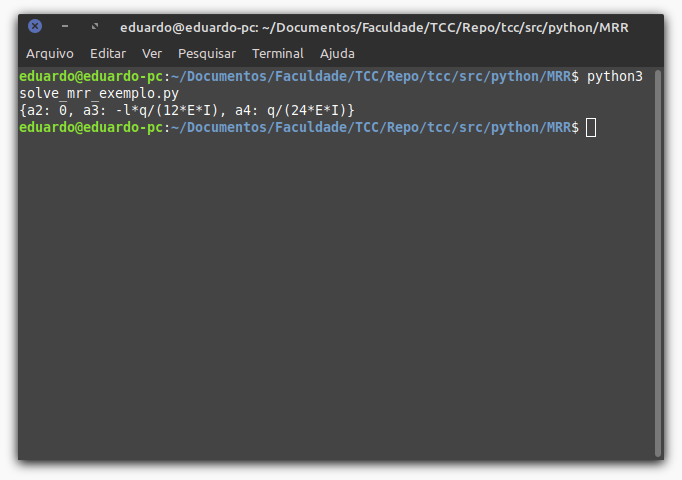
\includegraphics[scale=0.6]{../figuras/code/code_solve_mrr_exemplo_livro.png}
	\label{fig:code_solve_mrr_exemplo_livro}
	\legend{\ABNTEXfontereduzida Fonte: Elaborada pelo autor, 2019.}
\end{figure}

O valor de $a_1=-a_2l-a_3l^2-a_4l^3$ é determinado substituindo os valores de $a_2$, $a_3$ e $a_4$. Esse processo pode ser realizado de modo manual ou, mais rapidamente, utilizando a propria linguagem, adicionando o Código \ref{py_code_solve_mrr_isolatedcoef_ex_livro} ao final do Código \ref{py_code_solve_mrr_ex_livro}. Os comandos \textit{a1 = a1.subs(a2, sol[a2])} indica que a variável \textit{a1} receberá o valor de \textit{a1} substituindo o simbólo \textit{a2} pela solução do sistema encontrada no Código \ref{py_code_solve_mrr_ex_livro}.

\begin{lstlisting}[style=Python, xleftmargin=2em, numbers=left, firstnumber=13, caption={Código para a determinação do coeficiente $a_1$ do Exemplo \ref{ex:mrr_ex_livro}}, captionpos=t, label=py_code_solve_mrr_isolatedcoef_ex_livro]
a1 = -a2*l - a3*l**2 - a4 * l**3
a1 = a1.subs(a2, sol[a2])
a1 = a1.subs(a3, sol[a3])
a1 = a1.subs(a4, sol[a4])
print(a1)
\end{lstlisting}

{\color{red}É possível, ainda, construir uma função $v(x)$ utilizando os coeficientes $a_1$, $a_2$, $a_3$ e $a_4$ (O coeficiente $a_0$ foi ignorado devido ao seu valor ser nulo) com o Código \ref{py_code_solve_mrr_maxdef_ex_livro}. Utilizando, novamente, o comando \textit{subs} e a função definida no Código \ref{py_code_solve_mrr_maxdef_ex_livro}, pode-se calcular o valor de $v_3(x)$ em algum ponto, como, por exemplo, em $x=\dfrac{l}{2}$. De acordo com \citeonline{mefassan}, o valor $v_3(\frac{l}{2})$ é conhecido como o valor de máxima deflexão.}

\begin{lstlisting}[style=Python, xleftmargin=2em, numbers=left, firstnumber=18, caption={Código para a definição da função $v_3(x)$ do Exemplo \ref{ex:mrr_ex_livro}}, captionpos=t, label=py_code_solve_mrr_maxdef_ex_livro]
v = a1*x + sol[a2]*x**2 + sol[a3]*x**3 + sol[a4]*x**4
print(v)
maxdef = v.subs(x, l/2)
print(maxdef)
\end{lstlisting}

É importante observar, no Código \ref{py_code_solve_mrr_maxdef_ex_livro}, que ao construir a variável \textit{v} para representar a função, no primeiro coeficiente foi utilizado a variável \textit{a1}, enquanto que nas demais, foi utilizado \textit{sol[a2]}, \textit{sol[a3]} e \textit{sol[a4]}. Isso se deve ao fato de que os valores para os coeficientes $a_2$, $a_3$ e $a_4$ foram encontrados pela resolução do sistema, sendo a variável \textit{sol} a sua solução. Já, \textit{a1} foi definida como sendo a equação do termo $a_1$ isolado em função de $a_2$, $a_3$ e $a_4$.

Os Códigos \ref{py_code_solve_mrr_ex_livro}, \ref{py_code_solve_mrr_isolatedcoef_ex_livro} e \ref{py_code_solve_mrr_maxdef_ex_livro} são executados em sequência e, por essa razão, estão com numeração de linhas sequenciais: O Código \ref{py_code_solve_mrr_ex_livro} tendo as linhas de 1 a 12, o Código \ref{py_code_solve_mrr_isolatedcoef_ex_livro} de 13 a 17 e o Código \ref{py_code_solve_mrr_maxdef_ex_livro} de 18 a 21. A Figura \ref{fig:code_solve_mrr_exec_complete} mostra o resultado da execução dos Códigos \ref{py_code_solve_mrr_ex_livro}, \ref{py_code_solve_mrr_isolatedcoef_ex_livro} e \ref{py_code_solve_mrr_maxdef_ex_livro} no terminal.

\begin{figure}[h]
	\caption{Resultado apresentado pelos Códigos \ref{py_code_solve_mrr_ex_livro}, \ref{py_code_solve_mrr_isolatedcoef_ex_livro} e \ref{py_code_solve_mrr_maxdef_ex_livro}.}
	\centering
	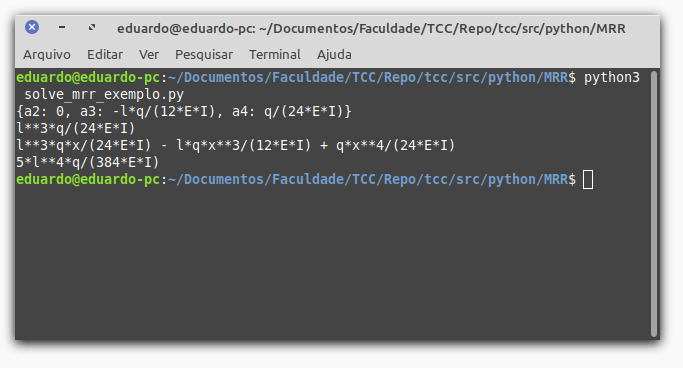
\includegraphics[scale=2]{../figuras/code/code_solve_mrr_exec_complete.png}
	\label{fig:code_solve_mrr_exec_complete}
	\legend{\ABNTEXfontereduzida Fonte: Elaborada pelo autor, 2019.}
\end{figure}

Observando, no terminal da Figura \ref{fig:code_solve_mrr_exec_complete}, pela ordem dos comandos \textit{print} executados no código, a primeira linha apresenta a solução do sistema, a segunda linha apresenta o valor do coeficiente $a_1$, a terceira linha apresenta a função $v_3(x)$ e a quarta linha apresenta o resultado de $v_3(\frac{l}{2})$ que é o valor de máxima deflexão da viga.

Ressaltando, novamente, que a escolha das funções de forma utilizadas na função aproximadora são de suma importância para o método de Rayleigh-Ritz. Para o uso de matemática simbólica, como nesse exemplo, deve-se tomar ainda mais cuidado com a escolha de tais funções pois, em alguns casos, a integração simbólica toma grande custo computacional. Em casos onde a integração simbólica se torna árdua, ou até mesmo impossível, o uso de algoritmos para integração numérica é necessário.

\section{Utilizando Funções Triangulares}

\citeonline{MRR_Deflex} apresenta o uso de funções triangulares como funções de forma, visando a discretização da função $y(x)$ exata. A função triangular trabalhada é definida como
\begin{equation}
	\label{eqn:cap_metodo_ray_ritz:tri_func_phi}
	\phi_i (x) = 
		\begin{cases}
			0 							& \mbox{se } 0 \leqslant x \leqslant x_{i - 1}\\
			\dfrac{x-x_{i-1}}{h_{i-1}} 	& \mbox{se } x_{i-1} < x \leqslant x_i\\
			\dfrac{x_{i+1}-x}{h_i}		& \mbox{se } x_i < x \leqslant x_{i+1}\\
			0							& \mbox{se } x_{i+1}<x\leqslant 1
		\end{cases}
	\text{,}
\end{equation}
onde $h_i = x_{i+1}-x_{i}$ e $h_{i-1}=x_i-x_{i-1}$. A Figura {\color{red}INSERIR FIGURA} apresenta uma ilustração da função $\phi_i(x)$ definida. A função exata, $y(x)$, que torna um funcional estacionário, é aproximado, então, por meio da função aproximadora
\begin{equation}
	\label{eqn:cap_metodo_ray_ritz:tri_func_app_v}
	v(x)=\sum_{i=1}^{n} a_i \phi_i(x)
	\text{.}
\end{equation}

Observe que, de acordo com a definição das funções de forma $\phi_i(x)$, a função $v(x)$, definida como combinação linear das $\phi_i(x)$, funcionará apenas para funcionais que dependem apenas de derivadas de primeira ordem, visto que a derivada de segunda ordem de qualquer $\phi_i(x)$ é nula.

A primeira derivada das funções $\phi_i(x)$ em relação a $x$ é escrita como
\begin{equation}
	\label{eqn:cap_metodo_ray_ritz:tri_func_phi_diff}
	\phi_i ' (x) = 
		\begin{cases}
			0 							& \mbox{se } 0 \leqslant x \leqslant x_{i - 1}\\
			\dfrac{1}{h_{i-1}} 			& \mbox{se } x_{i-1} < x \leqslant x_i\\
			\dfrac{-1}{h_i}				& \mbox{se } x_i < x \leqslant x_{i+1}\\
			0							& \mbox{se } x_{i+1}<x\leqslant 1
		\end{cases}
	\text{,}
\end{equation}
de onde a derivada de $v(x)$ em relação a $x$ é
\begin{equation}
	v'(x)=\sum_{i=1}^{n} a_i \phi_i '(x)
	\text{.}
\end{equation}

Considere o funcional
\begin{equation}
	\label{eqn:cap_metodo_ray_ritz:tri_func_funcional}
	I = \int_{0}^{1} \left [ 
		p(x) \left ( 
			\frac{dy}{dx} (x) 
		\right )^2
		+ q(x)(y(x))^2 
		- 2f(x)y(x) 
	\right ] dx
	\text{,}
\end{equation}
associado ao Problema de Valor de Contorno que modela a deflexão de uma viga apoiada sobre seus extremos. Pode-se, aqui, tomar $p(x)=e^x$, $q(x)=e^x$ e $f(x)=x+(2-x)e^x$ tendo em vista que a função exata $y(x)$ é conhecida, permitindo comparação. Aproximando $y(x)$ por meio da função $v(x)$ definida em \eqref{eqn:cap_metodo_ray_ritz:tri_func_app_v}, o funcional \eqref{eqn:cap_metodo_ray_ritz:tri_func_funcional} é escrito como
\begin{equation}
	\label{eqn:cap_metodo_ray_ritz:tri_func_funcional_approx}
	I = \int_{0}^{1} \left [
		p(x) \left (
			\sum_{i=1}^{n} a_i \phi_i '(x)
		\right )^2
		+ q(x) \left (
			\sum_{i=1}^{n} a_i \phi_i (x)
		\right )^2
		- 2f(x) \left (
			\sum_{i=1}^{n} a_i \phi_i (x)
		\right )
	\right ] dx
	\text{.}
\end{equation}

Para determinar os coeficientes $a_j$, as derivadas parciais de \eqref{eqn:cap_metodo_ray_ritz:tri_func_funcional_approx} em relação aos $a_j$ devem ser todas nulas, ou seja,
$$
	\frac{\partial I}{\partial a_j} = 0
	\text{,}
$$
onde $j=1$, $2$, $\dots$, $n$. Utilizando o Teorema \ref{teorema:regra_de_leibniz} (Regra de Leibniz),
\begin{equation}
	\label{eqn:cap_metodo_ray_ritz:tri_func_funcional_derivada}
	\frac{\partial I}{\partial a_j} = 
	\int_{0}^{1} \left [
		2p(x) \left (
			\sum_{i=1}^{n} a_i \phi_i'(x)
		\right ) \phi_j'(x)
		+ 2q(x) \left (
			\sum_{i=1}^{n} a_i \phi_i(x)
		\right ) \phi_j(x)
		- 2f(x)\phi_j(x)
	\right ] dx
	\text{.}
\end{equation}

Em \eqref{eqn:cap_metodo_ray_ritz:tri_func_funcional_derivada} foi utilizado o fato de que a derivada de $\displaystyle \sum_{i=1}^{n} a_i \phi_i(x)$ em relação a algum $a_j$, onde $1\leqslant j\leqslant n$, resulta em $\phi_j(x)$. O mesmo vale para a derivada de $\displaystyle \sum_{i=1}^{n} a_i \phi_i'(x)$ em relação a algum $a_j$, $1\leqslant j\leqslant n$, que resulta em $\phi_j'(x)$.

Manipulando as ordens de integração e de soma em \eqref{eqn:cap_metodo_ray_ritz:tri_func_funcional_derivada} tem-se
$$
	\frac{\partial I}{\partial a_j} = \sum_{i=1}^{n} \left (
		a_i \int_{0}^{1} \left [
			2p(x)\phi_i'(x)\phi_j'(x)
			+
			2q(x)\phi_i(x)\phi_j(x)
		\right ]
	\right )
	-
	\int_{0}^{1} 2f(x)\phi_j(x)dx
	\text{,}
$$
que, aplicando a condição $\dfrac{\partial I}{\partial a_j}=0$, resulta em um sistema de $n$ equações com $n$ incógnitas da forma
\begin{equation}
	\label{eqn:cap_metodo_ray_ritz:tri_func_sistema}
	\sum_{i=1}^{n} \left (
		a_i \int_{0}^{1} \left [
			2p(x)\phi_i'(x)\phi_j'(x)
			+
			2q(x)\phi_i(x)\phi_j(x)
		\right ] dx
	\right )
	=
	\int_{0}^{1} 2f(x)\phi_j(x)dx
	\text{,}
\end{equation}
onde $j=1$, $2$, $\dots$, $n$.

O sistema \eqref{eqn:cap_metodo_ray_ritz:tri_func_sistema} pode ser escrito na forma matricial $M\cdot A=B$, onde $M=[m_{j, i}]$ é a matriz de coeficientes, $A=[a_i]$ é a matriz coluna de incógnitas e $B=[b_j]$ é a matriz contendo os termos independentes. Assim, de \eqref{eqn:cap_metodo_ray_ritz:tri_func_sistema},
\begin{equation}
	\label{eqn:cap_metodo_ray_ritz:tri_func_mji}
	m_{j,i}=\int_{0}^{1} \left [
		2p(x)\phi_i'(x)\phi_j'(x)
		+
		2q(x)\phi_i(x)\phi_j(x)
	\right ]dx
	\text{,}
\end{equation}
\begin{equation}
	\label{eqn:cap_metodo_ray_ritz:tri_func_bj}
	b_j=\int_{0}^{1} 2f(x)\phi_j(x)dx
	\text{.}
\end{equation}

A partir de \eqref{eqn:cap_metodo_ray_ritz:tri_func_phi} e \eqref{eqn:cap_metodo_ray_ritz:tri_func_phi_diff}, os produtos $\phi_i(x)\phi_j(x)$ e $\phi_i'(x)\phi_j'(x)$ são não nulos apenas quando $i=j-1$, $i=j$ e $i=j+1$. Consequentemente, $m_{j,i}$ é não nulo apenas para $i=j-1$, $i=j$ e $i=j+1$.

O sistema $M\cdot A=B$ construido, pode ser resolvido, numericamente utilizando a linguagem de programação Python. Para tanto, o primeiro passo é importar os componentes a serem utilizados. No Código \ref{py_code_solve_mrr_tri_import} são importados os componentes \textit{numpy}, utilizado para a criação de alguns intervalos numéricos espaçados. Do pacote \textit{math} é importando a constante $e$. Do pacote \textit{sympy} é importado o método \textit{symbols} para a definição de símbolos matemáticos, de \textit{sympy.matrices} é importado o método \textit{zeros} para a criação de um matriz de tamanho determinado preenchida por números zeros e de \textit{sympy.solvers} é importado o método \textit{linsolve} utilizado para a resolução de sistemas lineares. Por último, é importado o pacote \textit{matplotlib.pyplot} como \textit{pyplot}\footnote{Utilizar o comando \textit{import matplotlib.pyplot as pyplot} faz com que, em vez de sempre escrever \textit{matplotlib.pyplot}, se possa escrever apenas \textit{pyplot} nos próximos comandos.} utilizado para plotar gráficos.

\begin{lstlisting}[style=Python, xleftmargin=2em, numbers=left, firstnumber=1, caption={Importação dos Pacotes Utilizados para a Resolução}, captionpos=t, label=py_code_solve_mrr_tri_import]
import numpy
from math import e
from sympy import symbols
from sympy.matrices import zeros
from sympy.solvers import linsolve
import matplotlib.pyplot as pyplot
\end{lstlisting}

Para o uso das funções de forma $\phi_i(x)$ e $\phi_i'(x)$, definidas em \eqref{eqn:cap_metodo_ray_ritz:tri_func_phi} e \eqref{eqn:cap_metodo_ray_ritz:tri_func_phi_diff}, respectivamente, é preciso criar um conjunto numérico espaçado (aqui o conjunto será igualmente espaçado, mas nada impede o uso de conjuntos com espaçamentos diferentes). Para a criação desse conjunto foi utilizada a função \textit{numpy.arange}, em Código \ref{py_code_solve_mrr_tri_interval}. No comando \textit{arange}. O uso do extremo $1.0001$ é apenas para garantir que o número $1$ esteja no conjunto gerado. A variável \textit{n} representa a quantidade de divisões a serem utilizadas no intervalo para a discretização da função exata.

\begin{lstlisting}[style=Python, xleftmargin=2em, numbers=left, firstnumber=7, caption={Criação dos intervalos numéricos}, captionpos=t, label=py_code_solve_mrr_tri_interval]
n = 5
space = 1/(n + 1)
intervals = numpy.arange(0, 1.0001, space)
\end{lstlisting}

\begin{lstlisting}[style=Python, xleftmargin=2em, numbers=left, firstnumber=10, caption={Função de forma $\phi$ e sua derivada}, captionpos=t, label=py_code_solve_mrr_tri_form_func]
def fi(i, x):
    if x <= intervals[i - 1]:
        return 0
    elif x <= intervals[i]:
        return ((x - intervals[i - 1]) / (intervals[i] - intervals[i - 1]))
    elif x <= intervals[i + 1]:
        return ((intervals[i + 1] - x) / (intervals[i + 1] - intervals[i]))
    else:
        return 0

def fi_diff(i, x):
    if x <= intervals[i - 1]:
        return 0
    elif x <= intervals[i]:
        return (1 / (intervals[i] - intervals[i - 1]))
    elif x <= intervals[i + 1]:
        return (1 / (intervals[i] - intervals[i + 1]))
    else:
        return 0
\end{lstlisting}

Numericamente, as funções $\phi_i(x)$ e $\phi_i'(x)$ foram programadas utilizando condicionais, em Código \ref{py_code_solve_mrr_tri_form_func}.

No Código \ref{py_code_solve_mrr_tri_form_func} o método utilizado para a integração numérica, que implementa a chamada regra do trapézio, é mostrado. Dentro do método, a variável \textit{steps} define em quantos intervalos o domínio de integração será dividido. Os parâmetros opcionais \textit{*args}, do método \textit{integrate}, são passados para a função a ser integrada, \textit{func}, e serão utilizados para passar os índices $i$ e $j$ quando necessário.

\begin{lstlisting}[style=Python, xleftmargin=2em, numbers=left, firstnumber=29, caption={Algoritmo para integração numérica usando a regra dos trapézios}, captionpos=t, label=py_code_solve_mrr_tri_integrate]
def integrate(func, start, end, *args):
    steps = 10000
    h = ((end - start) / steps)
    half = h / 2
    value = 0
    for i in range(0, steps):
        dh = func(start + h * i + half, *args)
        if i == 0 or i == (steps - 1):
            value += dh
        else:
            value += (2 * dh)
    return (value * (h / 2))
\end{lstlisting}

Para a integração numérica por meio do algoritmo implementado em Código \ref{py_code_solve_mrr_tri_integrate} é preciso definir funções com os integrandos de \eqref{eqn:cap_metodo_ray_ritz:tri_func_mji} e \eqref{eqn:cap_metodo_ray_ritz:tri_func_bj}. Essas funções são chamadas, no código, de \textit{m\underline{\hspace{.1in}}intern} e \textit{b\underline{\hspace{0.1in}}intern}, respectivamente. Na implementação do Código \ref{py_code_solve_mrr_tri_m_b}, os métodos \textit{m(i, j)} e \textit{b(i)} calculam os elementos das matrizes $M$ e $B$, respectivamente. Nesses métodos, é somado 1 aos índices $i$ e $j$ pois, na programação os elementos são indexados a partir de 0 e, na forma como definimos as funções de forma $\phi_i(x)$, elas são indexadas a partir de 1.

\begin{lstlisting}[style=Python, xleftmargin=2em, numbers=left, firstnumber=41, caption={Funções utilizadas para criação das matrizes do sistema linear}, captionpos=t, label=py_code_solve_mrr_tri_m_b]
def p(x):
    return e**x

def q(x):
    return e**x

def f(x):
    return (x+(2-x)*e**x)

def m_intern(x, i, j):
    return (p(x) * fi_diff(i, x) * fi_diff(j, x) + q(x) * fi(i, x) * fi(j, x))

def m(i, j):
    i = i + 1
    j = j + 1
    return integrate(m_intern, 0, 1, i, j)

def b_intern(x, i):
    return (f(x) * fi(i, x))

def b(i):
    i = i + 1
    return integrate(b_intern, 0, 1, i)
\end{lstlisting}

O próximo passo, consiste em criar a matriz aumentada do sistema, os símbolos que representam as incógnitas e, então, resolvê-lo. Isso é feito no Código \ref{py_code_solve_mrr_tri_solvesys}.

\begin{lstlisting}[style=Python, xleftmargin=2em, numbers=left, firstnumber=64, caption={Definição e resolução do sistema linear}, captionpos=t, label=py_code_solve_mrr_tri_solvesys]
M = zeros(n, n+1)
for i in range(0, n):
    M[i, n] = b(i)
    M[i, i] = m(i, i)
    if (i - 1) >= 0:
        M[i, i - 1] = m(i, i - 1)
    if (i + 1) < n:
        M[i, i + 1] = m(i, i + 1)
coeficients = symbols('a_0:{}'.format(n))
solution, = linsolve(M, coeficients)
\end{lstlisting}

A função $y(x)$ conhecida, exata, que torna o funcional de \eqref{eqn:cap_metodo_ray_ritz:tri_func_funcional_approx} estacionário é $y(x)=(x-1)(e^{-x}-1)$. Assim, utilizando a solução do Código \ref{py_code_solve_mrr_tri_solvesys} e a função exata $y(x)$, é possível criar funções, numéricas, representando a função exata e a função aproximada, plotando-as no mesmo gráfico, como feito no Código \ref{py_code_solve_mrr_tri_plot}.

\begin{lstlisting}[style=Python, xleftmargin=2em, numbers=left, firstnumber=74, caption={Plotagem das funções exata e aproximada}, captionpos=t, label=py_code_solve_mrr_tri_plot]
def function(solution, x):
    value = 0
    i = 0
    for c in solution:
        value += c * fi(i + 1, x)
        i = i + 1
    return value
def function_original(x):
    return ((x - 1) * (e**(-x) - 1))

plot_interval = numpy.arange(0.0, 1.0, 0.01)
plot_original = function_original(plot_interval)
plot_aprox = []
for i in plot_interval:
    plot_aprox.append(function(solution, i))
fig = pyplot.figure()
axes = fig.add_subplot(1, 1, 1)
axes.plot(plot_interval, plot_aprox, color='tab:blue')
axes.plot(plot_interval, plot_original, color='tab:orange')
axes.set_title('Rayleigh-Ritz With n=' + str(n))
pyplot.show()
\end{lstlisting}

Os Códigos \ref{py_code_solve_mrr_tri_import}, \ref{py_code_solve_mrr_tri_interval}, \ref{py_code_solve_mrr_tri_form_func}, \ref{py_code_solve_mrr_tri_integrate}, \ref{py_code_solve_mrr_tri_m_b}, \ref{py_code_solve_mrr_tri_solvesys} e \ref{py_code_solve_mrr_tri_plot} são sequênciais e devem ser executados dentro de um único arquivo, por isso suas numerações estão sequênciais. O resultado da execução do código para a resolução do sistema é mostrado na Figura \ref{fig:code_plot_mrr_triangulate}. Para maior precisão do método, pode-se aumentar o valor da variável \textit{n} do Código \ref{py_code_solve_mrr_tri_interval}, por exemplo, para 10. O gráfico plotado para $n=10$ é apresentado na Figura \ref{fig:code_plot_mrr_triangulate_n10}.

\begin{figure}[h]
	\caption{Resultado do método de Rayleigh-Ritz utilizando funções de forma triangulares com $n=5$.}
	\centering
	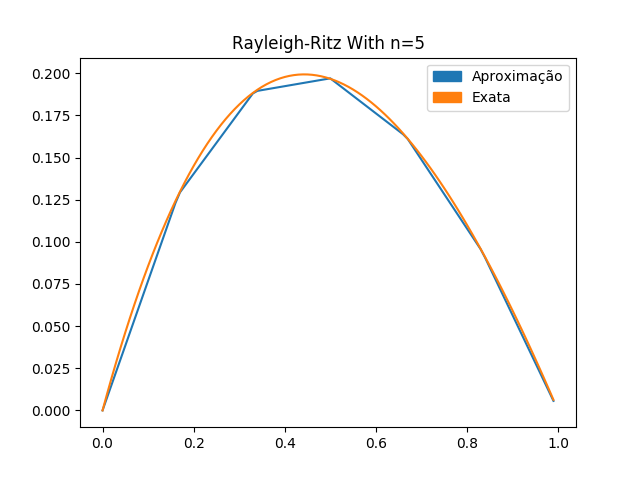
\includegraphics[scale=0.6]{../figuras/code/code_plot_mrr_triangulate.png}
	\label{fig:code_plot_mrr_triangulate}
	\legend{\ABNTEXfontereduzida Fonte: Elaborada pelo autor, 2019.}
\end{figure}

\begin{figure}[h]
	\caption{Resultado do método de Rayleigh-Ritz utilizando funções de forma triangulares com $n=10$.}
	\centering
	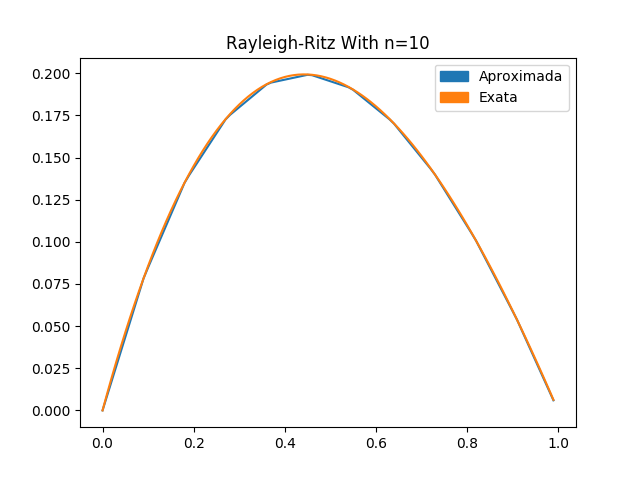
\includegraphics[scale=0.6]{../figuras/code/code_plot_mrr_triangulate_n10.png}
	\label{fig:code_plot_mrr_triangulate_n10}
	\legend{\ABNTEXfontereduzida Fonte: Elaborada pelo autor, 2019.}
\end{figure}

Quanto maior o valor da variável \textit{n} no Código \ref{py_code_solve_mrr_tri_interval} maior a precisão, porém, com maior custo computacional. Consequentemente, quanto maior o valor de \textit{n}, mais tempo o computador levará para a resolução do problema.

% ----------------------------------------------------------
% PARTE
% ----------------------------------------------------------
%\part{Preparação da pesquisa}
% ----------------------------------------------------------

% ---
% Capitulo com exemplos de comandos inseridos de arquivo externo 
% ---
%\include{abntex2-modelo-include-comandos}
% ---

% ----------------------------------------------------------
% PARTE
% ----------------------------------------------------------
%\part{Referenciais teóricos}
% ----------------------------------------------------------

\iffalse
% ---
% Capitulo de revisão de literatura
% ---
\chapter{Lorem ipsum dolor sit amet}
% ---

% ---
\section{Aliquam vestibulum fringilla lorem}
% ---

\lipsum[1]

\lipsum[2-3]

\lipsum[1]

\lipsum[2-3]

\lipsum[1]

\lipsum[2-3]

\lipsum[1]

\lipsum[2-3]

\lipsum[1]

\lipsum[2-3]

\lipsum[1]

\lipsum[2-3]

% ----------------------------------------------------------
% PARTE
% ----------------------------------------------------------
\part{Resultados}
% ----------------------------------------------------------

% ---
% primeiro capitulo de Resultados
% ---
\chapter{Lectus lobortis condimentum}
% ---

% ---
\section{Vestibulum ante ipsum primis in faucibus orci luctus et ultrices
posuere cubilia Curae}
% ---

\lipsum[21-22]

\subsection{TEstando subseção}

\subsubsection{Mais uma subseção.}

\subsubsubsection{ Chega de subsubseção.}


% ---
% segundo capitulo de Resultados
% ---
\chapter{Nam sed tellus sit amet lectus urna ullamcorper tristique interdum
elementum}
% ---

% ---
\section{Pellentesque sit amet pede ac sem eleifend consectetuer}
% ---

\lipsum[24]

% ----------------------------------------------------------
% Finaliza a parte no bookmark do PDF
% para que se inicie o bookmark na raiz
% e adiciona espaço de parte no Sumário
% ----------------------------------------------------------
\phantompart

% ---
% Conclusão
% ---
\chapter{Conclusão}
% ---

\lipsum[31-33]

\fi

% ----------------------------------------------------------
% ELEMENTOS PÓS-TEXTUAIS
% ----------------------------------------------------------
\postextual
% ----------------------------------------------------------

% ----------------------------------------------------------
% Referências bibliográficas
% ----------------------------------------------------------
\bibliography{../references}

% ----------------------------------------------------------
% Glossário
% ----------------------------------------------------------
%
% Consulte o manual da classe abntex2 para orientações sobre o glossário.
%
%\glossary

% ----------------------------------------------------------
% Apêndices
% ----------------------------------------------------------

% ---
% Inicia os apêndices
% ---
\begin{apendicesenv}

% Imprime uma página indicando o início dos apêndices
\partapendices

% Apêndice A
\chapter{Conceitos de Análise no $\mathbb{R}^n$}
\label{apend:regra_de_leibniz}
{
	Durante o desenvolvimento dos resultados do texto, tais como a obtenção da equação de Euler-Lagrange, é necessário o uso de alguns conceitos e resultados de Análise no $\mathbb{R}^n$. Estes conceitos serão trabalhados neste apêndice, tomando como referência \citeonline{analise_elon2}.

	\begin{definicao}
		Um conjunto $K\subset \mathbb{R}^n$ é compacto se, e somente se, toda sequência de pontos em $K$ possui uma subsequência que converge para um ponto de $K$.
	\end{definicao}

	\begin{teorema}
		\label{teorema:func_uniformemente}
		Seja $f:X\times K \longrightarrow \mathbb{R}^n$ contínua, onde $X\subset \mathbb{R}^m$, para algum $m$, e $K$ é compacto. Fixemos $x_0 \in X$. Para todo $\varepsilon > 0$, existe um $\delta > 0$ tal que $x\in X$, $|x-x_0|<\delta \Longrightarrow |f(x, \alpha)-f(x_0,\alpha)|<\varepsilon$, seja qual for $\alpha \in K$.
		\begin{proof}
		Suponha que o teorema não seja válido, então existiriam $\varepsilon > 0$ e sequências de pontos $x_k\in X$, $\alpha_k \in K$ tais que $|x_k-x_0|<\frac{1}{k}$ e $|f(x_k,\alpha_k)-f(x_0,\alpha_k)|\geqslant \varepsilon$. Passando a uma subsequência, se necessário e admitindo que $\lim \alpha_k=\alpha \in K$, devido ao fato de que o conjunto $K$ é compacto.
		
		Como, $|x_k-x_0|<\frac{1}{k}$, $-\frac{1}{k}<x_k-x_0<\frac{1}{k}$, então, $x_0-\frac{1}{k}<x_k<x_0+\frac{1}{k}$, e, como $\lim \left (x_0-\frac{1}{k} \right ) = x_0$ e $\lim \left ( x_0 + \frac{1}{k} \right )=x_0$, então, $\lim x_k=x_0$. Devido a continuidade de $f$ tem-se $\varepsilon \leqslant \lim |f(x_k,\alpha_k)-f(x_0,\alpha _k)|=|f(x_0,\alpha)-f(x_0,\alpha)|=0$, uma contradição, pois da hipótese $\varepsilon >0$.
		\end{proof}
	\end{teorema}
	
	\begin{teorema}[Derivação sob o sinal de integral ou Regra de Leibniz]
		\label{teorema:regra_de_leibniz}
		Dado $U\subset \mathbb{R}^n$, aberto, seja $f:U\times[a,b]\longrightarrow \mathbb{R}$ uma função com as seguintes propriedades:
		\begin{enumerate}
			\item Para todo $x \in U$, a função $x \longmapsto f(x,t)$ é integrável em $a \leqslant t \leqslant b$.
			\item A $i$-ésima derivada parcial $\frac{\partial f}{\partial x_i}(x,t)$ existe para cada $(x,t)\in U\times [a,b]$ e a função $\frac{\partial f}{\partial x_i}:U\times [a,b]\longrightarrow \mathbb{R}$ assim definida é contínua.
		\end{enumerate}
		Então a função $\varphi: U\longrightarrow \mathbb{R}$ dada por
		$$\varphi(x)=\int_a^b f(x,t)dt\text{,}$$
		possui $i$-ésima derivada parcial em cada ponto $x\in U$, sendo
		$$\frac{\partial \varphi}{\partial x_i}(x)=\int_a^b \frac{\partial f}{\partial x_i}(x,t)dt\text{.}$$

		\begin{proof}
			Considere
			$$
			\frac{\varphi(x+se_i)-\varphi(x)}{s}
			=
			\int_a^b \frac{f(x+se_i, t)-f(x,t)}{s} dt\text{,}
			$$
			de onde subtraindo $\displaystyle \int_a^b \frac{\partial f}{\partial x_i}(x,t) dt$ de ambos os lados, tem-se
			\begin{equation}
			\label{eqn:cap_ap_leibniz:subtract_1}
			\frac{\varphi(x+se_i)-\varphi(x)}{s}
			- \int_a^b \frac{\partial f}{\partial x_i}(x,t) dt
			=
			\int_a^b \left [ 
				\frac{f(x+se_i, t)-f(x,t)}{s} 
				- \frac{\partial f}{\partial x_i}(x,t)
			\right ] dt
			\end{equation}
			
			Pelo Teorema do Valor Médio para funções reais, existe $\theta \in [0,1]$ de modo que
			$$
				\frac{f(x+se_i,t)-f(x,t)}{s}=\frac{\partial f}{\partial x_i}(x+\theta s e_i,t)\text{,}
			$$
			onde $\theta \in [0,1]$ garante que $\theta s$ esteja entre $]0, s[$, satisfazendo as condições do Teorema do Valor Médio. Assim, de \eqref{eqn:cap_ap_leibniz:subtract_1} tem-se
			%donde pode-se escrever \eqref{eqn:cap_ap_leibniz:subtract_1} como
			\begin{equation}
				\label{eqn:cap_ap_leibniz:tvm}
				\frac{\varphi(x+se_i)-\varphi(x)}{s}
				- \int_a^b \frac{\partial f}{\partial x_i}(x,t) dt
				=
				\int_a^b \left [
					\frac{\partial f}{\partial x_i}(x+\theta s e_i, t)-\frac{\partial f}{\partial x_i}(x,t)
				\right ] dt\text{.}
			\end{equation}
			
			Como $\dfrac{\partial f}{\partial x_i}$ é contínua e $[a,b]$ é compacto, pelo Teorema \ref{teorema:func_uniformemente}, para todo $\varepsilon > 0$, existe um $\delta > 0$, de modo que
			\begin{equation}
				\label{eqn:cap_ap_leibniz:compact_limit}
				|s|<\delta \Longrightarrow
				\left | 
					\frac{\partial f}{\partial x_i} (x+\theta s e_i, t) - \frac{\partial f}{\partial x_i}(x,t)
				\right | < \frac{\varepsilon}{b-a}
			\end{equation}
			seja qual for $t \in [a,b]$.
			
			Usando o fato de que $\displaystyle \Big |\int_a^b f(x)dx \Big | \leqslant \int_a^b |f(x)| dx$, obtêm-se
			$$
			\left |
				\int_a^b \left [
					\frac{\partial f}{\partial x_i}(x+\theta s e_i, t)-\frac{\partial f}{\partial x_i}(x,t)
				\right ] dt
			\right |
			\leqslant
			\int_a^b\left |
				\frac{\partial f}{\partial x_i}(x+\theta s e_i, t)-\frac{\partial f}{\partial x_i}(x,t)
			\right | dt\text{,}
			$$
			e, utilizando \eqref{eqn:cap_ap_leibniz:compact_limit}, tem-se a inequação
			$$
			\left |
				\int_a^b \left [
					\frac{\partial f}{\partial x_i}(x+\theta s e_i, t)-\frac{\partial f}{\partial x_i}(x,t)
				\right ] dt
			\right |
			<
			\int_a^b \frac{\varepsilon}{b-a} dt
			$$
			\begin{equation}
				\label{eqn:cap_ap_leibniz:epsilon_limit}
				\left |
					\int_a^b \left [
						\frac{\partial f}{\partial x_i}(x+\theta s e_i, t)-\frac{\partial f}{\partial x_i}(x,t)
					\right ] dt
				\right |
				< \varepsilon \text{.}
			\end{equation}
			
			De \eqref{eqn:cap_ap_leibniz:tvm} e \eqref{eqn:cap_ap_leibniz:epsilon_limit}, verifica-se que
			$$
				|s|<\delta \Longrightarrow
				\left |
					\frac{\varphi(x+se_i)-\varphi(x)}{s}
					- \int_a^b \frac{\partial f}{\partial x_i}(x,t) dt
				\right |
				< \varepsilon\text{,}
			$$
			que é, a definição formal do limite
			$$
				 \lim_{s\to 0} \frac{\varphi (x+se_i)-\varphi(x)}{s}= \int_a^b \frac{\partial f}{\partial x_i} (x, t)dt \text{,}
			$$
			ou seja,
			$$
				\frac{\partial \varphi}{\partial x_i}(x)=\int _a^b \frac{\partial f}{\partial x_i}(x,t)dt\text{.}
			$$
		\end{proof}
	\end{teorema}
	
	\begin{definicao}
		\label{def:cap_conceitos_analise:classe_ck}
		Seja o aberto $U\subset\mathbb{R}^n$. Uma função $f:U\longrightarrow\mathbb{R}$ é dita de classe $C^0$ quando é contínua. Diz-se, também, que $f:U\longrightarrow\mathbb{R}$ é de classe $C^1$ quando existem, em cada ponto $x\in U$, as derivadas parciais $\dfrac{\partial f}{\partial x_1}(x)$, $\dots$, $\dfrac{\partial f}{\partial x_n}(x)$ e, as $n$ funções $\dfrac{\partial f}{\partial x_i}:U\longrightarrow \mathbb{R}$, assim definidas, são contínuas. Mais geralmente, uma função $f:U\longrightarrow\mathbb{R}$ é dita de classe $C^k$, onde $k>0$ é um inteiro, quando ela possuir derivadas parciais em todos os pontos de $U$ e as funções $\dfrac{\partial f}{\partial x_i}$, $\dots$, $\dfrac{\partial f}{\partial x_n}:U\longrightarrow \mathbb{R}$ forem de classe $C^{k-1}$.
	\end{definicao}
	
	A Definição \ref{def:cap_conceitos_analise:classe_ck} é equivalente a dizer que uma função $f:U\longrightarrow\mathbb{R}$, onde $U\subset\mathbb{R}^n$, é dita de classe $C^k$ se todas as suas derivadas parciais até a ordem $k$ existirem e, ainda, forem todas contínuas. Completando, $f$ será de classe $C^0$ caso seja contínua.
}

\chapter{Resolução de Sistemas Lineares Utilizando a Linguagem Python}
\label{apend:res_sis_lin}
{
	O sistema linear com matriz aumentada \eqref{eqn:cap_metodo_ray_ritz:matriz_sistema} pode ser facilmente resolvido utilizando métodos trabalhados em Álgebra Linear, como, por exemplo, o método de Gauss-Jordan. Outra forma de se resolver o sistema é fazendo o uso da linguagem de programação Python.
	
	Deste modo, seja, o sistema com matriz aumentada \eqref{eqn:cap_metodo_ray_ritz:matriz_sistema}
	\begin{equation}
		\label{eqn:cap_ap_sis_lin:matriz_sistema}
		\begin{amatrix}{3}
			2 & 3l  & 4l^2 				 & C \\
			1 & 2l  & 3l^2				 & \frac{1}{2}C \\
			8 & 18l & \frac{144}{5} l^2 & D
		\end{amatrix}
		\text{,}
	\end{equation}
	onde 
	\begin{equation}
		\label{eqn:cap_ap_sis_lin:aux_var_C}
		C=-\frac{ql^2}{12EI}
		\text{,}
	\end{equation}
	e
	\begin{equation}
		\label{eqn:cap_ap_sis_lin:aux_var_D}
		D=-\frac{3ql^2}{10EI}
		\text{.}
	\end{equation}
	
	Para a resolução do sistema usando Python é necessário, primeiro, importar alguns componentes da biblioteca SymPy:
	\begin{lstlisting}[style=Python]
from sympy import symbols, Matrix
from sympy.solvers import linsolve
	\end{lstlisting}
	
	Serão importados os componentes \textit{symbols} para permitir a definição de símbolos matemáticos, \textit{Matrix} para a manipulação de matrizes e, finalmente, \textit{linsolve} para a resolução de sistemas lineares.
	
	Para a definição do sistema, utilizaremos os mesmos símbolos, $l$, $C$, e $D$, que são definidos, dentro da linguagem, utilizando o comando \textit{symbols} importado:
	\begin{lstlisting}[style=Python]
l, C, D = symbols('l C D')
	\end{lstlisting}
	
	A matriz aumentada é definida utilizando o componente \textit{Matrix} importado. Cada uma de suas linhas é escrita como um Array contendo os elementos das colunas. A matriz é escrita, então, como um Array de linhas.
	\begin{lstlisting}[style=Python]
A = Matrix([
    [2, 3 * l ,  4 * l**2      ,  C  ],
    [1, 2 * l ,  3 * l**2      ,  C/2],
    [8, 18 * l,  144 / 5 * l**2,  D  ]
])
	\end{lstlisting}
	
	A resolução do sistema é feita pelo método \textit{linsolve} já importado. Primeiro, definimos três novos símbolos, $a_1$, $a_2$ e $a_3$ que são as incógnitas do sistema e então, executamos o método passando como argumento a matriz $A$ definida e os símbolos.
	\begin{lstlisting}[style=Python]
a2, a3, a4 = symbols("a2 a3 a4")
sol, = linsolve(A, [a2, a3, a4])
print(sol)
	\end{lstlisting}

	\begin{figure}[h]
		\caption{Execução do Código para a Resolução do Sistema Linear.}
		\centering
		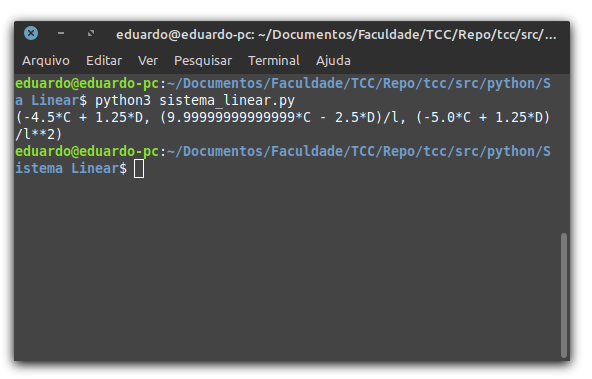
\includegraphics[scale=2.5]{../figuras/code/code_solve_sis_linear.png}
		\label{fig:code_solve_sis_linear}
		\legend{\ABNTEXfontereduzida Fonte: Elaborada pelo autor, 2019.}
	\end{figure}
	
	O comando \textit{print(sol)} exibe a solução do sistema linear, como um Array (Veja Figura \ref{fig:code_solve_sis_linear}). O primeiro valor do Array corresponde a incógnita $a_2$, o segundo valor a $a_3$ e o último valor a $a_4$. Assim, $a_2=-4.5C+1.25D$, $a_3=\dfrac{1}{l}(10C-2.5D)$ e $a_4=\dfrac{1}{l^2}(-5C+1.25D)$. Pode-se converter os números decimais para frações obtendo
	\begin{equation}
		\label{eqn:cap_ap_sis_lin:result_a2}
		a_2=\frac{5}{4}D-\frac{9}{2}C
		\text{,}
	\end{equation}
	\begin{equation}
		\label{eqn:cap_ap_sis_lin:result_a3}
		a_3=\frac{1}{l}\left (
			10C - \frac{5}{2} D
		\right ) \text{,}
	\end{equation}
	\begin{equation}
		\label{eqn:cap_ap_sis_lin:result_a4}
		a_4=\frac{1}{l^2}\left (
			\frac{5}{4}D-5C
		\right ) \text{.}
	\end{equation}
	
	Substituindo $C$ e $D$, de \eqref{eqn:cap_ap_sis_lin:aux_var_C} e \eqref{eqn:cap_ap_sis_lin:aux_var_D}, em \eqref{eqn:cap_ap_sis_lin:result_a2}, \eqref{eqn:cap_ap_sis_lin:result_a3} e \eqref{eqn:cap_ap_sis_lin:result_a4} e simplificando os valores obtem-se a solução do sistema
	$$
		a_2 = 0\text{,}
	$$
	$$
		a_3 = -\frac{ql}{12EI}\text{,}
	$$
	$$
		a_4 = \frac{q}{24EI}\text{.}
	$$

	O código completo utilizado para a resolução do sistema linear com matriz aumentada \eqref{eqn:cap_ap_sis_lin:matriz_sistema} é apresentado em Código \ref{py_code_solve_sys_linear}.
		
	\begin{lstlisting}[style=Python, xleftmargin=2em, numbers=left, caption=Resolução de Sistemas Lineares em Python, captionpos=t, label=py_code_solve_sys_linear]
from sympy import symbols, Matrix
from sympy.solvers import linsolve

l, C, D = symbols('l C D')

A = Matrix([
    [2, 3 * l ,  4 * l**2      ,  C  ],
    [1, 2 * l ,  3 * l**2      ,  C/2],
    [8, 18 * l,  144 / 5 * l**2,  D  ]
])

a2, a3, a4 = symbols("a2 a3 a4")
sol, = linsolve(A, [a2, a3, a4])

print(sol)
	\end{lstlisting}
}

\end{apendicesenv}
% ---

\iffalse
% ----------------------------------------------------------
% Anexos
% ----------------------------------------------------------

% ---
% Inicia os anexos
% ---
\begin{anexosenv}

% Imprime uma página indicando o início dos anexos
\partanexos

% ---
\chapter{Morbi ultrices rutrum lorem.}
% ---
\lipsum[30]

% ---
\chapter{Cras non urna sed feugiat cum sociis natoque penatibus et magnis dis
parturient montes nascetur ridiculus mus}
% ---

\lipsum[31]

% ---
\chapter{Fusce facilisis lacinia dui}
% ---

\lipsum[32]

\end{anexosenv}

\fi

%---------------------------------------------------------------------
% INDICE REMISSIVO
%---------------------------------------------------------------------
\phantompart
\printindex
%---------------------------------------------------------------------

\end{document}
